%!TEX root = ../plos_template.tex

\section{Biological network architecture}\label{sec:covergenotypespace}
A module of a biological network is represented by a subset of variables, $O \subseteq L$. A biological network architecture, $\mathcal{G}$, may then be represented by a subset of all possible such modules. This is to say that $\mathcal{G}$ is a subset of the set of all subsets of $L$, $\mathcal{G} \subseteq \mathcal{P}(L)$, that satisfies the following two conditions
\begin{enumerate}
\item $\cup_i O_i = \cup \mathcal{G} = L$,
\item If $O,O' \in \mathcal{G}$ and $O \subseteq O'$ then $O = O'$.
\end{enumerate}
The first condition is just a statement that $\mathcal{G}$ represents a decomposition of the collection of all variables under consideration into subsets and this is why we refer to $\mathcal{G}$ as a collection of biological network modules. The second condition means simply that we will not consider nested subsets and so we will take for our $O \in \mathcal{G}$ the biggest $O \in \mathcal{G}$ that is not a subset of some other $O' \in \mathcal{G}$. The second condition also implies that if a given subset of variables $O'$ is compatible in a sense to be explained more precisely in what proceeds then any smaller subset of variables $O$ is also compatible.

Mathematically, the two conditions given above state that $\mathcal{G}$ is a \emph{covering} of the set $L$.  This is equivalent to $(L, \mathcal{G})$ being a reduced hypergraph, Sperner family, or clutter over $L$ \cite{Lauritzen1996}.  Coverings $\mathcal{G}$ of the space of biological network variables contain the necessary information to make precise what we heuristically refer to at other points in this paper as modularity in order to cohere with standard terminology in systems biology literature while attempting to submit our own precise interpretation of the relatively colloquial concept.

\section{Functorial formulation of probability distributions over network modules}\label{secsupp:probabilitydistributionsonnetworks}

As stated in \ref{sec:probabilitydistributionsonnetworks}, in addition to the expression state of the whole genome, we usually will be interested in the expression states of portions of the genome that interact either directly or indirectly.  We will represent these portions as subsets of $L$ and their expression states as functions from these subsets to $P$.

The power set of $L$, which we shall denote as $\mathcal{P}(L)$, can be regarded  as a category~\cite{Lane1998,MacLane1992,Awodey2006,Abramsky2011} in which the objects are subsets of $L$ and morphisms represent inclusion of a smaller subset into a larger superset (i.e. $O \subseteq O' \Rightarrow O \rightarrow O'$).  Then we will represent our expression states of subsets by the functor $\expr = \mathrm{Hom}(-,P)$.  Specifically, this functor may be described as
\begin{equation}\label{eq:gpfunctor}
\begin{split}
\expr \colon (\mathcal{P}(L), \subseteq) &\to \mathbf{Set} \\
O &\mapsto P^O,\\
O \subseteq O' &\mapsto (S \in P^{O'} \mapsto \{e|_O \mid e \in S\}). % res^{O'}_{O}.
\end{split}
\end{equation}
For example, if we consider the case in which we have two variables $L=\{l_1,l_2\}$ and there are two potential states, $P=\{0,1\}$, then $\expr$ operates on the lattice of subsets generated by $L$ to give spaces of functions containing the possible \gnpm{} as exemplified in \ref{fig:efunctor}.
% If we consider the case in which we have two variables $L=\{l_1,l_2\}$ and there are two states, $P=\{0,1\}$, then $\expr$ operates on each of the possible subsets of $L$ (i.e. $\{\}$, $\{l_1\}$, $\{l_2\}$, $\{l_1,l_2\}$) to give spaces of functions containing the possible \gnpm{} as exemplified in \ref{fig:efunctor}.
For example, $\mathcal{E}(\{l_1,l_2\}) = \{ e^{12}_{00},e^{12}_{01},e^{12}_{10},e^{12}_{11} \}$ where $e^{12}_{01}(l_1) = 0$ and $e^{12}_{01}(l_2) = 1$. As another example, $\mathcal{E}(\{l_1\}) = \{ e^{1}_{0},e^{1}_{1} \}$ where $e^{1}_{0}(l_1)=0$ and $e^{1}_{1}(l_1)=1$. $\expr ( \{ l_1 \} \! \subseteq \! \{ l_1, l_2 \} )$ is given explicitly by
\begin{equation}
\begin{aligned}
e^{12}_{00} \mapsto e^{1}_{0}\\
e^{12}_{01} \mapsto e^{1}_{0}\\
e^{12}_{10} \mapsto e^{1}_{1}\\
e^{12}_{11} \mapsto e^{1}_{1}
\end{aligned}.
\end{equation}

Next, we introduce extended probability distributions by defining a functor $\mathcal{D}$ that will compose with $\mathcal{E}$ to convert collections of \gnpm{} into probability distributions over them.  Given a finite set $S$, define $\dist(S)$ to be the set of all maps from $S$ to the interval $[0,1]$ which satisfy the following two conditions:  For all $d \in \dist(S)$, we have $d(S) \in \{0,1\}$.\footnote{Normally, we would only have $d(S) = 1$, but since we want to introduce conditionalization in a coherent way it becomes necessary to admit degenerate distributions where $d(S) = 0$ as well. This simplifies the exposition by not requiring us to worry about dividing by zero and having to introduce special cases when dealing with conditional probabilities and partial functions.  Of course, it also means that we cannot automatically assume that an element of $\dist(S)$ can be normalized without checking this fact but in our examples, this verification will turn out to be routine and trivial.}  For all  $d \in \dist(S)$ and all $A, B \subset S$, we have $d(A) + d(B) = d(A \cup B) + d(A \cap B)$.

Returning to the running example,
$$\mathcal{D}(\mathcal{E}(\{l_1,l_2\})) = \{p^{12}_{00},p^{12}_{01},p^{12}_{10},p^{12}_{11} \mid p^{12}_{00} \geq 0, p^{12}_{01} \geq 0,p^{12}_{10} \geq 0,p^{12}_{11} \geq 0, p^{12}_{00} + p^{12}_{01} + p^{12}_{10} + p^{12}_{11} = 1 \},$$
$$\mathcal{D}(\mathcal{E}(\{l_1\})) = \{p^{1}_{0}, p^{1}_{1} \mid p^{1}_{0} \geq 0, p^{1}_{1} \geq 0, p^{1}_{0}+p^{1}_{1} = 1 \}.$$

If $S$ and $S'$ are finite sets, which in our case will usually be sets of \gnpm{} given by $\mathcal{E}(O)$, $d \in \dist(S)$ and $d' \in \dist(S')$ are probability distributions over these spaces, and $f \colon S \to S'$ is a partial function, we will say that $f$ is compatible with $d$ and $d'$ when, for all $X \in \mathrm{img}(f)$, we have
\begin{equation}
 d'(X) =
  \begin{cases}
    \frac{d'(\mathrm{img}(f))}{d(\mathrm{dom}(f))}d(f^{-1}(X)) & d(\mathrm{dom}(f)) \neq 0, \\
    0 & d(\mathrm{dom}(f)) = 0.
  \end{cases}
\end{equation}
In other words, the map $f$ preserves ratios of probabilities of events.  In the case where $f$ is a partial surjection $(\mathrm{img}(f)=S')$, compatibility completely determines $d'$ in terms of $d$ and thus $\dist$ may be regarded as a functor from the subcategory of sets with partial surjections as morphisms to transformations on probability distributions:
\begin{equation}\label{eq:distfunctor}
 d' = \dist(f)(d) =
  \begin{cases}
    X \mapsto \frac{d(f^{-1}(X))}{d(\mathrm{dom}(f))} & d(\mathrm{dom}(f)) \neq 0, \\
    X \mapsto 0 & d(\mathrm{dom}(f)) = 0.
  \end{cases}
\end{equation}
Specifically, when $f$ is a total surjection, this map corresponds to marginalization. For example, in the case $f = \expr ( \{ l_1 \} \! \subseteq \! \{ l_1, l_2 \} )$
\begin{equation}\label{eq:dfunctorex}
\begin{split}
\dist \big(\expr ( \{ l_1 \} \! \subseteq \! \{ l_1, l_2 \} ) \big) \colon \expr ( \{ l_1 \} \! \subseteq \! \{ l_1, l_2 \} ) &\to \expr ( \{ l_1 \} ), \\
d &\mapsto d',
\end{split}
\end{equation}
then
\begin{equation}\label{eq:margexample}
d\hspace{.09em}'(\{e^1_0\}) = \dist (f)(d)(\{e^1_0\}) = \frac{d(f^{-1}(\{ e^1_0\}))}{d(\{ e^{12}_{00},e^{12}_{01},e^{12}_{10},e^{12}_{11} \})} = \frac{d(\{ e^{12}_{00},e^{12}_{01}\})}{1} = d( \{ e^{12}_{00} \} ) + d( \{ e^{12}_{01} \} ) = p^{12}_{00} + p^{12}_{01}.
\end{equation}
When $f$ is a partial isomorphism, it corresponds to conditionalization. For example, if $f$ is defined such that we condition on variable one being in state zero, $l_1 = 0$,
\begin{equation}
f \colon \{ e^{12}_{00} , e^{12}_{01} \} \subset \expr ( \{ l_1, l_2 \} ) \to \{ f(e^{12}_{00}) , f(e^{12}_{01}) \}
\end{equation}
then
\begin{equation}\label{eq:condexample}
d\hspace{.09em}'(\{ f(e^{12}_{00}) \} ) = \dist (f)(d)( \{ f(e^{12}_{00}) \}) = \frac{d( f^{-1}( \{ f(e^{12}_{00}) \}) )}{d(\{ e^{12}_{00},e^{12}_{01} \})} = \frac{d(\{ e^{12}_{00} \})}{d( \{ e^{12}_{00} \} ) + d( \{ e^{12}_{01} \} )} = \frac{p^{12}_{00}}{p^{12}_{00} + p^{12}_{01}}.
\end{equation}
Finally, when $f$ is a general partial surjection, it corresponds to a combination of conditionalization and marginalization.

In order to admit the basic tools of linear algebra for the purpose of calculations regarding relationships between spaces of probability distributions we explain how they embed into linear spaces. By definition, an extended probability distribution $p \in \dist(S)$ is an element of $\mathbb{R}^S$. We denote the inclusion map as
\begin{equation}\label{eq:emb}
\rm{emb}(S) : \dist(S) \to \mathbb{R}^S.
\end{equation}
Because a convex combination of two probability distributions is again a probability distribution, the image of $\mathrm{emb}(S)$ consists of a convex set and the origin point (corresponding to the degenerate zero distribution).  Furthermore, if $n$ is the number of elements of the set $S$, this convex set works out to be the probability simplex with $n$ vertices, which we denote $\Delta_{n-1}$.  In our example above, $\mathcal{D}(\mathcal{E}(\{l_1,l_2\}))$ is the tetrahedron $\Delta_3$. Since any vector $v \in \mathbb{R}^S$ may be written as $v = c_{+} p_{+} - c_{-} p_{-}$ where $c_{+}, c_{-} \in [0,\infty)$ and $p_{+}$ and $p_{-}$ are probability distributions, the image of $\mathrm{emb}(S)$ spans the vector space $\mathbb{R}^S$.  For purposes of later reference, note that, if $f \colon S \to S'$ is a partial surjection, then $\mathcal{D}$ extends to a fractional linear map, as in \ref{eq:condexample}, from $\mathbb{R}^S$ to $\mathbb{R}^{S'}$ and that, in the special case where $f$ is a total surjection, as in \ref{eq:margexample}, it is in fact a linear map.

\section{Precise formulation of coarse-graining network states}\label{secsupp:coarsegrainingphenotypes}

As described in \ref{sec:genenetworkphenmap} it is also possible to consider network states that derive from coarse-graining lower-level network states. Once this is done, one arrives at probability distributions over network modules like that introduced in \ref{sec:probabilitydistributionsonnetworks}. As a result of this, our conclusions that are formulated in terms of a single level of coarse-graining \gnpm{} also apply to coarse-graining over multiple levels at once despite the fact that the parameters of the relevant probabilistic model are likely to be different.

% For a subset of genes $O \subseteq L$, let $\phi_i (O)$ be the set of phenotype values at level $i$, which can be determined from the expression levels of genes in $O$.  Note that $\phi_i (O)$ may be empty if the set $O$ does not contain enough genes to determine the values of any phenotype at level $i$. If $i \le j$, let $\Omega_{ij}(O) : \phi_i(O) \to \phi_j(O)$ be the coarse-graining map which describes how higher level phenotypes are determined from lower level phenotypes. This map is formulated precisely in \refsupp{} \ref{secsupp:coarsegrainingphenotypes}.

% Recall from \ref{sec:coarsegrainingphenotypes} that

For each subset of variables $O \in \mathcal{P}(L)$, let $\phi_i (O)$ be the set of network states at level $i$, which can be determined from the expression levels of variables in $O$.  Note that $\phi_i (O)$ may be empty if the set $O$ does not contain enough variables to determine the values of any network state at level $i$. When $O_1 \subseteq O_2 \in \mathcal{P}(L)$, we have a restriction map $\pi_i^{O_2 O_1} \colon \phi_i(O_2) \to \phi_i(O_1)$.  These maps satisfy the consistency conditions that $\pi_i^{OO}$ is the identity map and that $\pi_i^{O_3 O_2} \circ \pi_i^{O_2 O_1} = \pi_i^{O_3 O_1}$, i.e. $\pi_i$ is a functor on $(\mathcal{P}(L), \subseteq)$.  As stated earlier, we set $\phi_1 (O) = P^O$ and $\pi_1^{O_2 O_1}$ to be the restriction map from $P^{O_2}$ to $P^{O_1}$.  If $i \le j$, let $\Omega_{ij}(O) : \phi_i(O) \to \phi_j(O)$ be the coarse-graining map which describes how higher level network states are determined from lower level network states.  These maps are all surjections and, for consistency, we will require the following conditions:
\begin{enumerate}
\item $\Omega_{ij}(O) \circ \Omega_{jk}(O) = \Omega_{ik}(O)$ whenever $i \le j \le k$.
\item $\Omega_{ii}(O)$ is the identity map on $\phi_i (O)$.
\item If $O_1 \subseteq O_2 \in \mathcal{P}(L)$ and $i > j$, then $\Omega_{ij}(O_1) \circ \pi_i^{O_2 O_1} = \pi_j^{O_2 O_1} \circ \Omega_{ij}(O_2)$
\end{enumerate}
In other words, $\Omega$ must be suitably functorial in both of its arguments.

For example, if our lower level network states for a set of variables $O_1 = \{ l_1,l_2,l_3,l_4 \}$ are given by a set of binary sequences, then the projection of these network states down to the set $O_2 = \{l_3,l_4\}$ followed by mapping to the higher level network states $x=\{01,10\}$ and $y=\{11\}$ is equivalent to first mapping to the higher-level network states $X$ and $Y$ and then projecting down to $O_2$ shown by the equivalent paths from the top-left to the bottom-right in \ref{fig:phenotypehierarchy}A.
Of course, there is an equivalent diagram for the subset $\{ l_1,l_2,l_3 \}$.

Since the map $\Omega_{1i}(O)$ is a surjection from $P^O$ onto $\phi_i(O)$, we can use it to map our probabilistic structures to $\phi_i(O)$.  Set $\mathcal{E}_i = \Omega_{1i}(O)^{-1} \circ \mathcal{E}$ and $\dist_i = \Omega_{1i}(O)^{-1} \circ \dist$.  Then we end up with the overall relationships summarized in \ref{fig:abstractroadmap}. As a consequence of the consistency conditions the coarse-graining maps $\phi$ and $\Omega$, there is a natural transformation between the functors $\expr_i$ and $\expr_{i+1}$ implying that the following diagram commutes
$$
\xymatrix{
\expr_{i+1}(O_1) \ar[r]^{\expr_{i+1}(\subseteq)} \ar[d]_{t_{O_1}} & \expr_{i+1}(O_2) \ar[d]^{t_{O_2}} \\
\expr_{i}(O_1) \ar[r]^{\expr_{i}(\subseteq)} & \expr_{i}(O_2) }
$$
for any $O_2 \subseteq O_1$.

Given a covering $\mathcal{G}$ of the space of biological network variables, we can consider the higher order network states associated to the elements of $\mathcal{G}$.  For a suitable choice of cover and a suitable level of network states, it may happen that the network states associated to different elements of $\mathcal{G}$ are distinct.  For instance, in the example of \ref{fig:phenotypehierarchy}, if we take $\mathcal{G} = \{O_1, O_2\}$ where $O_1 = \{l_1, l_2, l_3\}$ and $O_2 = \{l_3, l_4\}$, we have $\phi_{i+1}(O_1) = \{u,v\}$ and $\phi_{i+1}(O_2) = \{x,y\}$.  In such a case, if we were to perform one experiment which measured the network states $\{u,v\}$ and another experiment which measured $\{x,y\}$, then the result could be understood as examining the covering $\{O_1, O_2\}$ at network state level $i+1$.



\section{Sheaf-theoretic formulation of compatibility of distributions on \gnpm{}}\label{secsupp:compatibilityofgpms}

% \section{Compatibility of distributions on \gnpm{}}\label{sec:compatibilityofgpms}
Given a covering of the space of variables $\mathcal{G}$, a compatible family for $\mathcal{G}$ with respect to $\mathcal{D} \circ \mathcal{E}$ is given by a family of distributions $\dist{}(\expr{}(\mathcal{G})) = \{d_O \in \dist (\mathcal{E}(O)) | O \in \mathcal{G}\}$ such that for all $O, O' \in \mathcal{G}$
\begin{eqnarray}\label{eq:sheafcond}
%\forall O \in \mathcal{G} \left[ \exists d_O \in \mathcal{D}_R\mathcal{E}(O) \right],\\
d_O|O \cap O' = d_{O'}|O \cap O'.
\end{eqnarray}
This first set of conditions is later referred to as local consistency. The space of all such locally consistent distributions for a given covering, $\mathcal{G}$, is referred to as $\mathbb{L}(\mathcal{G})$ where
\begin{equation}
\mathbb{L}(\mathcal{G}) = \{ d_O  \in \dist{}(\expr{}(\mathcal{G})) \mid (\forall O,O' \in \mathcal{G})\,\, d_O|O \cap O' = d_O'|O \cap O' \}.
\end{equation}
These conditions mean that any two distributions $d_O$ and $d_{O'}$ in the \emph{compatible family} of distributions marginalize to the same disribution over the intersection of $O$ with $O'$. If these constraints are not satisfied, then there is no way to make a consistent assignment of probabilities to the states of even a single variable. In this case one of the constraints will be eliminated or duplication of a variable may allow for the independent satisfaction of both constraints.

If, moreover, this first condition implies the existence of $d \in \mathcal{D}( \mathcal{E}(L))$ such that $d|O = d_O$ for all $O \in \mathcal{G}$ then the system is said to satisfy the global consistency condition. The space of all such globally consistent distributions for a given covering, $\mathcal{G}$, is referred to as $\mathbb{M}(\mathcal{G})$ where
\begin{equation}
\mathbb{M}(\mathcal{G}) = \{ d_O \in \dist{}(\expr{}(\mathcal{G})) \mid (\exists d ) \,\, d|O = d_O \}.
\end{equation}
In general, the system of equations $d|O = d_O$ for all $O \in \mathcal{G}$ is underdetermined and so local consistency does not imply global consistency. The local and global consistency conditions are related to the mathematical concepts from which they derive in \refsupp{} \ref{secsupp:compatibilityofgpms}. We will now examine the situation more closely to determine under what circumstances global consistency holds.

For a cover of the space of variables, $\mathcal{G}$, we can construct a matrix, $\mathbf{G}$, representing the relationship,
% $R = \coprod_{O \in \mathcal{G}} \mathcal{E}(O \subset L) \subseteq \mathcal{E}(L) \times \expr (\mathcal{G})$,
between \gnpm{} having as domain particular network modules given by the $O \in \mathcal{G}$ and those global \gnpm{} defined on $L$.
% We would like to construct the matrix representation of $\mathbf{G}$. In the first factor, $\mathcal{E}(L) = P^L = \{e^{L}_{\vec{j}} | \vec{j} \in P^{|L|}\}$.
%%$\{t_1, \ldots t_m\} = \{t_j | t_j \in P^L\}$.
% For the second factor, $ \mathcal{E}(\mathcal{G}) = \coprod_{O \in \mathcal{G}} \mathcal{E}(O) = \{e^O_{\vec{i}} | O \in \mathcal{G}, \vec{i} \in P^{|O|} \}$.
% %$\{e_1, \ldots e_n\} = \coprod_{O \in \mathcal{G}} \mathcal{E}(O)$.
%  So we have two sets of maps, one defined on $P^L$ and the other defined on $\mathcal{E}(O) = P^O$ for each $O \in \mathcal{G}$. This yields a method of specifying the intended relationship that defines
$\mathbf{G}$ can be specified for all $e^O_{\vec{i}} \in \mathcal{E}(\mathcal{G})$ and $e^{L}_{\vec{j}} \in \mathcal{E}(L)$:
\begin{eqnarray}\label{eq:margmat}
\mathbf{G}(e^O_{\vec{i}},e^L_{\vec{j}}) =
\begin{cases}
1, & e^L_{\vec{j}}|O = e^O_{\vec{i}},\\
0, & \text{otherwise}.
\end{cases}
\end{eqnarray}
For example, given the covering $\mathcal{G} = \{ \{l_1\}, \{l_2\} \}$ of a set of two variables $L = \{ l_1, l_2 \}$ the associated matrix $\mathbf{G}$ is shown in \ref{fig:efunctor}B.

% Combining the marginalization matrix $\mathbf{G}$ with the maps previously defined in \ref{eq:emb} the following diagram demonstrates the relationships between the spaces of probability distributions and the linear spaces in which they are embedded

% \begin{equation*}
% \xymatrix{
%  \mathbb{R}^{\mathcal{E}(L)} \ar[r]^{\mathbf{G}} &
%    \mathbb{R}^{\mathcal{E}(\mathcal{G})} \\
%  \dist (\mathcal{E}(L)) \ar[r]^{\mathbf{G}} \ar@{^{(}->}[u]^{emb_{\mathcal{E}(L)}}& \ar@{^{(}->}[u]_{emb_{\mathcal{E}(\mathcal{G})}}
%   \dist (\mathcal{E}(\mathcal{G}))
%   }
% \end{equation*}
The locally, $\mathbb{L}(\mathcal{G})$, and globally, $\mathbb{M}(\mathcal{G})$, consistent polytopes correspond to the spaces of probability distributions satisfying the local and global consistency conditions described above. The globally consistent polytope is a subspace of the locally consistent one. This is because an ostensible inverse to $\mathbf{G}$ is underdetermined and can only be estimated in general (most commonly using the maximum entropy principle).
% In terms of the diagram $\mathbb{M}(\mathcal{G})$ is given by $\mathbf{G}(emb_{\mathcal{E}(L)}(\mathcal{D}(\mathcal{E}(L))))$ and $\mathbb{L}(\mathcal{G})$ is given by $emb_{\mathcal{E}(\mathcal{G})}(\mathcal{D}(\mathcal{E}(\mathcal{G}))) \cap \mathbf{G}(\mathbb{R}^{\mathcal{E}(L)})$, where
% \begin{eqnarray}
% emb_{\mathcal{E}(\mathcal{G})}(\mathcal{D}(\mathcal{E}(\mathcal{G}))) &=& \left\{ p^{O}_{\vec{i}} \; \bigg| \; (\forall\, O \in \mathcal{G}) \; (\forall\, \vec{i} \in P^{|O|}) \;\; p^O_{\vec{i}} \geq 0, \; (\forall\, O \in \mathcal{G}) \sum_{\vec{i} \in P^{|O|}} p^{O}_{\vec{i}} = 1 \right\},\\
% emb_{\mathcal{E}(L)}(\mathcal{D}(\mathcal{E}(L))) &=& \left\{ p^L_{\vec{i}} \; \bigg| \; (\forall\, \vec{i} \in P^{|L|}) \; p^L_{\vec{i}} \geq 0, \; \sum_{\vec{i} \in P^{|L|}} p^L_{\vec{i}} = 1 \right\}.
% \end{eqnarray}
To determine explicit conditions on the probabilities we express $\mathbb{L}(\mathcal{G})$ and $\mathbb{M}(\mathcal{G})$ in terms of the fundamental subspaces associated to the linear map $\mathbf{G}$. In order for a vector $v$ to lie in $\mathbf{G}(\mathbb{R}^{\mathcal{E}(L)})$, we must have $v=\mathbf{G}x$ for some $x \in \mathbb{R}^{\mathcal{E}(L)}$.  The cokernel of $\mathbf{G}$ gives the obstructions to this system $v=\mathbf{G}x$ having a solution. In order to eliminate these obstructions, constraints must be imposed on $\mathbb{R}^{\mathcal{E}(\mathcal{G})}$ and these constraints are given precisely via annihilating the cokernel, i.e. $\mathbf{G}(\mathbb{R}^{\mathcal{E}(L)}) = \{ v \; | \; (\forall u \in coker \mathbf{G}) \; u \cdot v = 0\}$.  We then take the appropriate intersection to determine $\mathbb{L}(\mathcal{G})$ by requiring $v \in \mathcal{D}(\mathcal{E}(\mathcal{G}))$
\begin{eqnarray}\label{eq:localpolytope}
\mathbb{L}(\mathcal{G}) &=& \{ v \in \dist{}(\expr{}(\mathcal{G})) \; | \; (\forall u \in coker \mathbf{G}) \; u \cdot v = 0\}.
\end{eqnarray}
Since $\mathbf{G}$ is not invertible the equation $v = \mathbf{G}x$ can only be solved up to an element of $ker \mathbf{G}$. $v = \mathbf{G}x$ can thus be solved on a subspace $T$ of $\mathbb{R}^{\mathcal{E}(L)}$ such that $T \oplus ker \mathbf{G} = \mathbb{R}^{\mathcal{E}(L)}$ to yield
\begin{eqnarray}\label{eq:globalpolytope}
\mathbb{M}(\mathcal{G}) &=& \{ v \; | v = \mathbf{G} x,\; (\exists x \in T) \; (\exists y \in \dist{}(\expr{}(L)))\; x-y \in ker \mathbf{G}  \}.
\end{eqnarray}
In order to obtain inequalities that define $\mathbb{M}(\mathcal{G})$, Fourier-Motzkin elimination can be used to eliminate $x$ and $y$. Alternatively one can use the fact, \cite{Wainwright2007} proposition 8.3, that $\mathbb{M}(\mathcal{G})$ is given by removing the non-integer vertices from a vertex represntation of $\mathbb{L}(\mathcal{G})$ and the ability to interconvert between vertex and inequality representations to compute the same inequalities as described in \refsupp{} \ref{secsupp:fourcycleexample}.

Recall from \ref{sec:compatibilityofgpms} that given a covering of the space of variables $\mathcal{G}$, a compatible family for $\mathcal{G}$ with respect to $\mathcal{D} \circ \mathcal{E}$ is given by a family of distributions $\{d_O \in \dist (\mathcal{E}(O)) | O \in \mathcal{G}\}$ such that for all $O, O' \in \mathcal{G}$
\begin{eqnarray}
%\forall O \in \mathcal{G} \left[ \exists d_O \in \mathcal{D}_R\mathcal{E}(O) \right],\\
d_O|O \cap O' = d_{O'}|O \cap O'.
\end{eqnarray}
This first set of conditions is later referred to as local consistency. These conditions mean that any two distributions $d_O$ and $d_{O'}$ in the \emph{compatible family} of distributions marginalize to the same disribution over the intersection of $O$ with $O'$.

If, moreover, this first condition implies the existence of $d \in \mathcal{D}( \mathcal{E}(L))$ such that $d|O = d_O$ for all $O \in \mathcal{G}$ then the system is said to satisfy the global consistency condition.  This latter condition is also referred to as the \emph{sheaf condition}.  $\mathcal{E}$ alone turns out to be a sheaf because it satisfies the analogous conditions: for $\{e_O \in \mathcal{E}(O) | O \in \mathcal{G}\}$ such that $e_{O_{1}} | O_1 \cap O_2 = e_{O_{2}} | O_1 \cap O_2$ there exists $e \in \mathcal{E}(\cup_{O \in \mathcal{G}} O)$ such that $e_O = e|O$ for all $O \in \mathcal{G}$.  However, for $\dist \circ \mathcal{E}$ the sheaf condition is not automatically satisfied and it only defines a presheaf.  We will now examine the situation more closely to determine under what circumstances global consistency holds.

For a cover of the space of variables, $\mathcal{G}$, we can construct a matrix, $\mathbf{G}$, representing the relationship, $R = \coprod_{O \in \mathcal{G}} \mathcal{E}(O \subset L) \subseteq \mathcal{E}(L) \times \expr (\mathcal{G})$, between \gnpm{} having as domain particular network modules given by the $O \in \mathcal{G}$ and those global \gnpm{} defined on $L$. We would like to construct the matrix representation of $\mathbf{G}$. In the first factor, $\mathcal{E}(L) = P^L = \{e^{L}_{\vec{j}} | \vec{j} \in P^{|L|}\}$.
%$\{t_1, \ldots t_m\} = \{t_j | t_j \in P^L\}$.
For the second factor, $ \mathcal{E}(\mathcal{G}) = \coprod_{O \in \mathcal{G}} \mathcal{E}(O) = \{e^O_{\vec{i}} | O \in \mathcal{G}, \vec{i} \in P^{|O|} \}$.
%$\{e_1, \ldots e_n\} = \coprod_{O \in \mathcal{G}} \mathcal{E}(O)$.
 So we have two sets of maps, one defined on $P^L$ and the other defined on $\mathcal{E}(O) = P^O$ for each $O \in \mathcal{G}$. This yields the method of specifying the intended relationship that defines $\mathbf{G}$ for all $e^O_{\vec{i}} \in \mathcal{E}(\mathcal{G})$ and $e^{L}_{\vec{j}} \in \mathcal{E}(L)$ given in \ref{eq:margmat}.
This matrix can be viewed as an operator acting via matrix multiplication on distributions
\begin{eqnarray*}
\mathbf{G} \colon \mathcal{D}(\mathcal{E}(L)) &\rightarrow& \mathcal{D}( \mathcal{E}(\mathcal{G})),\\
d &\mapsto& \coprod_{O \in \mathcal{G}} d|O,
\end{eqnarray*}
and thereby taking a global distribution, $\dist (\mathcal{E}(L))$, defined on \gnpm{} whose domain is the full set of variables $L$ into the local distributions, $\dist (\mathcal{E}(\mathcal{G}))$, that are defined relative to network modules contained in a covering of the space of variables $\mathcal{G}$. $\mathbf{G}$ provides a way of determining the distributions on \gnpm{} for a given context (i.e. $\coprod_{O \in \mathcal{G}} d|O$) that can be derived from distributions (i.e. $\mathcal{D} ( \mathcal{E}(L) )$) defined on the global \gnpm{} (i.e. $\mathcal{E}(L)$ as opposed to $\mathcal{E}(O)$).

Combining the marginalization matrix $\mathbf{G}$ with the maps previously defined in \ref{eq:emb} the following diagram demonstrates the relationships between the spaces of probability distributions and the linear spaces in which they are embedded

\begin{equation*}
\xymatrix{
 \mathbb{R}^{\mathcal{E}(L)} \ar[r]^{\mathbf{G}} &
   \mathbb{R}^{\mathcal{E}(\mathcal{G})} \\
 \dist (\mathcal{E}(L)) \ar[r]^{\mathbf{G}} \ar@{^{(}->}[u]^{emb_{\mathcal{E}(L)}}& \ar@{^{(}->}[u]_{emb_{\mathcal{E}(\mathcal{G})}}
  \dist (\mathcal{E}(\mathcal{G}))
  }
\end{equation*}
The locally, $\mathbb{L}(\mathcal{G})$, and globally, $\mathbb{M}(\mathcal{G})$, consistent polytopes embedded within $\mathbb{R}^{\mathcal{E}(\mathcal{G})}$ correspond to the spaces of probability distributions satisfying the local and global consistency conditions described above. The globally consistent polytope is a subspace of the locally consistent one. This is because an ostensible inverse to $\mathbf{G}$ is underdetermined and can only be estimated in general (most commonly using the maximum entropy principle). In terms of the diagram $\mathbb{M}(\mathcal{G})$ is given by $\mathbf{G}(emb_{\mathcal{E}(L)}(\mathcal{D}(\mathcal{E}(L))))$ and $\mathbb{L}(\mathcal{G})$ is given by $emb_{\mathcal{E}(\mathcal{G})}(\mathcal{D}(\mathcal{E}(\mathcal{G}))) \cap \mathbf{G}(\mathbb{R}^{\mathcal{E}(L)})$, where
\begin{eqnarray}
emb_{\mathcal{E}(\mathcal{G})}(\mathcal{D}(\mathcal{E}(\mathcal{G}))) &=& \left\{ p^{O}_{\vec{i}} \; \bigg| \; (\forall\, O \in \mathcal{G}) \; (\forall\, \vec{i} \in P^{|O|}) \;\; p^O_{\vec{i}} \geq 0, \; (\forall\, O \in \mathcal{G}) \sum_{\vec{i} \in P^{|O|}} p^{O}_{\vec{i}} = 1 \right\}, \label{eq:embdeg}\\
emb_{\mathcal{E}(L)}(\mathcal{D}(\mathcal{E}(L))) &=& \left\{ p^L_{\vec{i}} \; \bigg| \; (\forall\, \vec{i} \in P^{|L|}) \; p^L_{\vec{i}} \geq 0, \; \sum_{\vec{i} \in P^{|L|}} p^L_{\vec{i}} = 1 \right\}. \label{eq:embdel}
\end{eqnarray}
If the embedding into linear spaces is to be considered explicitly, then \ref{eq:embdeg} and \ref{eq:embdel} can be substituted for $\dist{}(\expr{}(\mathcal{G}))$ and $\dist{}(\expr{}(L))$ in \ref{eq:localpolytope} and \ref{eq:globalpolytope}.
% To determine explicit conditions on the probabilities we express these in terms of the fundamental subspaces associated to the linear map $\mathbf{G}$. In order for a vector $v$ to lie in $\mathbf{G}(\mathbb{R}^{\mathcal{E}(L)})$, we must have $v=\mathbf{G}x$ for some $x \in \mathbb{R}^{\mathcal{E}(L)}$.  The cokernel of $\mathbf{G}$ gives the obstructions to this system $v=\mathbf{G}x$ having a solution. In order to eliminate these obstructions, constraints must be imposed on $\mathbb{R}^{\mathcal{E}(\mathcal{G})}$ and these constraints are given precisely via annihilating the cokernel, i.e. $\mathbf{G}(\mathbb{R}^{\mathcal{E}(L)}) = \{ v \; | \; (\forall u \in coker \mathbf{G}) \; u \cdot v = 0\}$.  We then take the appropriate intersection to determine $\mathbb{L}(\mathcal{G})$ by requiring $v \in emb_{\mathcal{E}(\mathcal{G})}(\mathcal{D}(\mathcal{E}(\mathcal{G})))$
% \begin{eqnarray}\label{eq:localpolytope}
% \mathbb{L}(\mathcal{G}) &=& \{ v \in emb_{\mathcal{E}(\mathcal{G})}(\mathcal{D}(\mathcal{E}(\mathcal{G}))) \; | \; (\forall u \in coker \mathbf{G}) \; u \cdot v = 0\}.
% \end{eqnarray}
% Since $\mathbf{G}$ is not invertible the equation $v = \mathbf{G}x$ can only be solved up to an element of $ker \mathbf{G}$. $v = \mathbf{G}x$ can thus be solved on a subspace $T$ of $\mathbb{R}^{\mathcal{E}(L)}$ such that $T \oplus ker \mathbf{G} = \mathbb{R}^{\mathcal{E}(L)}$ to yield
% \begin{eqnarray}\label{eq:globalpolytope}
% \mathbb{M}(\mathcal{G}) &=& \{ v \; | v = \mathbf{G} x,\; (\exists x \in T) \; (\exists y \in emb_{\mathcal{E}(L)}(\mathcal{D}(\mathcal{E}(L))))\; x-y \in ker \mathbf{G})  \}.
% \end{eqnarray}
% In order to obtain inequalities that define $\mathbb{M}(\mathcal{G})$, Fourier-Motzkin elimination can be used to eliminate $x$ and $y$. Alternatively one can use the fact, \cite{Wainwright2007} proposition 8.3, that $\mathbb{M}(\mathcal{G})$ is given by removing the non-integer vertices from a vertex represntation of $\mathbb{L}(\mathcal{G})$ and the ability to interconvert between vertex and inequality representations to compute the same inequalities as described in the \refsupp{}.

\subsection{Example of apparent satisfaction of unsatisfiable constraints}\label{secsupp:apparentinconsistency}
The inequalities defining $\mathbb{M}(\mathcal{G})$ were derived under the assumption that the two-element probabilities were obtained by mariginalizing a three-element distribution.  If some other procedure, such as conditionalization, is used to obtain them instead, these inequalities need not apply. For example, suppose now that $L = \{l_1,l_2,l_3 \}$, $P = \{0,1,2\}$, $\mathcal{G} = \{\{l_1,l_2\},\{l_2,l_3\},\{l_3,l_1\}\}$ where we have simply added an element to $P$ relative to the example described above. In the previous example the marginal maps were given by $\dist (\expr (O \subset L))$ with one for each $O \in \mathcal{G}$. If we combine these marginal maps with conditioning on one out of the three genes being in state two and each of the other two being in states zero or one, then we have instead $\dist (\pi_1), \dist (\pi_2), \dist (\pi_3)$ where $\pi_1 = \expr (\{l_1,l_2\} \subset L)|\{ e^{123}_{ij2} \mid i,j \in \{ 0,1 \} \},\; \pi_2 = \expr (\{l_2,l_3\} \subset L)|\{ e^{123}_{2ij} \mid i,j \in \{ 0,1 \} \},\; \pi_3 = \expr (\{l_3,l_1\} \subset L)|\{ e^{123}_{i2j} \mid i,j \in \{ 0,1 \} \}$. In this case, if we have the following assignment of probabilities for a distribution $d$
\begin{equation}\label{eq:condprobs}
\begin{aligned}
p^{123}_{002} &= 1/30 & p^{123}_{020} &= 2/15 & p^{123}_{200} &= 2/15\\
p^{123}_{012} &= 2/15 & p^{123}_{021} &= 1/30 & p^{123}_{201} &= 1/30\\
p^{123}_{102} &= 2/15 & p^{123}_{120} &= 1/30 & p^{123}_{210} &= 1/30\\
p^{123}_{112} &= 1/30 & p^{123}_{121} &= 2/15 & p^{123}_{211} &= 2/15
\end{aligned}
\end{equation}
with all other probabilities being zero, then $\dist (\pi_1)(d), \dist (\pi_2)(d), \dist (\pi_3)(d)$ are equivalent to the probability tables in \ref{fig:inconsistentthreecycle}A, which as shown in \ref{sec:inconsistency}, could not be achieved by marginalization alone. For example, given that $dom(\pi_1) = \{ e^{123}_{002}, e^{123}_{012}, e^{123}_{102}, e^{123}_{112} \}$ then $d(dom(\pi_1)) = \frac{1}{30} + \frac{2}{30} + \frac{2}{30} + \frac{1}{30} = \frac{1}{3}$. Substituting this factor and the fact that ${\pi_1}^{-1}(e^{12}_{ij}) = e^{123}_{ij2}$ into \ref{eq:distfunctor}
$$
p^{12}_{ij} = \dist (\pi_1)(d)(e^{12}_{ij}) = \frac{d({\pi_1}^{-1}(e^{12}_{ij}))}{d(dom(\pi_1))} = 3 p^{123}_{ij2},
$$
then renormalizes probabilities resulting in $p^{12}_{00} = 0.1, p^{12}_{01} = 0.4, p^{12}_{10} = 0.4, p^{12}_{11} = 0.1$ along with the analogs for $p^{23}_{ij}$ and $p^{13}_{ij}$, which are precisely equivalent to what appears in \ref{fig:inconsistentthreecycle}A as suggested above.

If constraints consistent with those of \ref{fig:inconsistentthreecycle}A are placed on the given network, either the network must add another variable in order to satisfy them directly or the network context imposing those constraints must coarse-grain the network in a suitable way. In what follows, we argue that the former is much more plausible than the latter. This ultimately suggests conditions in which cycle breakage may be selected for to relieve inconsistent constraints that can arise when cycles are present.


\section{Example volume ratio computation for the four-cycle network architecture}\label{secsupp:fourcycleexample}

For the purposes of this example, we take the full set of variables to be $L = \{ l_1,l_2,l_3,l_4 \}$. Consider the case in which each of the network modules under consideration has two variables and we specify the covering of the space of variables given by $\mathcal{G} = \{\{l_1,l_2 \},\{l_1,l_4 \},\{l_3,l_2\},\{l_3,l_4\} \}$.  We will compute $\mathbb{L}(\mathcal{G})$ using the same method which was used for the example of three variables.  By analogy with \ref{eq:localconsistencythreegenes}, the local consistency conditions now are as follows:
\begin{equation}
\begin{aligned}\label{eq:pparsys}
p^1_0 &= p^{12}_{00} + p^{12}_{01} = p^{14}_{00} + p^{14}_{01}, &
p^1_1 &= p^{12}_{10} + p^{12}_{11} = p^{14}_{10} + p^{14}_{11},\\
p^3_0 &= p^{32}_{00} + p^{32}_{01} = p^{34}_{00} + p^{34}_{01},&
p^3_1 &= p^{32}_{10} + p^{32}_{11} = p^{34}_{11} + p^{34}_{11},\\
p^2_0 &= p^{12}_{00} + p^{12}_{10} = p^{32}_{00} + p^{32}_{10},&
p^2_1 &= p^{12}_{01} + p^{12}_{11} = p^{32}_{01} + p^{32}_{11},\\
p^4_0 &= p^{14}_{00} + p^{14}_{10} = p^{34}_{00} + p^{34}_{10},&
p^4_1 &= p^{14}_{01} + p^{14}_{11} = p^{34}_{01} + p^{34}_{11}.
\end{aligned}
\end{equation}
Likewise, the equations determined by the conditions $v = \mathbf{G}(x)$ which are analogous to the matrix $\mathbf{G}$ in \ref{fig:efunctor}B are now
\begin{equation}
\begin{aligned}\label{eq:globsys}
p^{12}_{00} &= p^{1234}_{0000} + p^{1234}_{0010} + p^{1234}_{0001} + p^{1234}_{0011} &
p^{12}_{10} &= p^{1234}_{1000} + p^{1234}_{1010} + p^{1234}_{1001} + p^{1234}_{1011} \\
p^{12}_{01} &= p^{1234}_{0100} + p^{1234}_{0110} + p^{1234}_{0101} + p^{1234}_{0111} &
p^{12}_{11} &= p^{1234}_{1100} + p^{1234}_{1110} + p^{1234}_{1101} + p^{1234}_{1111} \\
p^{14}_{00} &= p^{1234}_{0000} + p^{1234}_{0001} + p^{1234}_{1000} + p^{1234}_{1001} &
p^{14}_{10} &= p^{1234}_{0010} + p^{1234}_{0011} + p^{1234}_{1010} + p^{1234}_{1011} \\
p^{14}_{01} &= p^{1234}_{0100} + p^{1234}_{0101} + p^{1234}_{1100} + p^{1234}_{1101} &
p^{14}_{11} &= p^{1234}_{0110} + p^{1234}_{0111} + p^{1234}_{1110} + p^{1234}_{1111} \\
p^{32}_{00} &= p^{1234}_{0000} + p^{1234}_{0010} + p^{1234}_{0100} + p^{1234}_{0110} &
p^{32}_{10} &= p^{1234}_{1000} + p^{1234}_{1010} + p^{1234}_{1100} + p^{1234}_{1110} \\
p^{32}_{01} &= p^{1234}_{0001} + p^{1234}_{0011} + p^{1234}_{0101} + p^{1234}_{0111} &
p^{32}_{11} &= p^{1234}_{1001} + p^{1234}_{1011} + p^{1234}_{1101} + p^{1234}_{1111}\\
p^{34}_{00} &= p^{1234}_{0000} + p^{1234}_{1000} + p^{1234}_{0100} + p^{1234}_{1100} &
p^{34}_{10} &= p^{1234}_{0010} + p^{1234}_{1010} + p^{1234}_{0110} + p^{1234}_{1110} \\
p^{34}_{01} &= p^{1234}_{0001} + p^{1234}_{1001} + p^{1234}_{0101} + p^{1234}_{1101} &
p^{34}_{11} &= p^{1234}_{0011} + p^{1234}_{1011} + p^{1234}_{0111} + p^{1234}_{1111},
\end{aligned}
\end{equation}
which are displayed in matrix form in \ref{tab:logmat222}.

Rather than proceeding to compute $\mathbb{L}(\mathcal{G})$ using elimination of inequalities as before, we will instead make use of the fact that the extremal points of $\mathbb{L}(\mathcal{G})$ happen to be the extremal points of $\mathbb{L}(\mathcal{G})$ with integer coordinates.  This is the approach which was used to compute the volume ratios shown in \ref{fig:ncycvolrat}.  More specifically, those computations were done using a computer program based on the following algorithm which is available via a virtual machine that can be reconstructed using the instructions available on \href{https://github.com/cameronraysmith/sep}{github}:

\begin{enumerate}
\item Compute (a basis for) the cokernel of $\mathbf{G}$. The cokernel gives the obstructions to the system $\mathbf{G}\mathbf{X}=\mathbf{V}$ having a solution. In order to eliminate these obstructions constraints must be imposed on $\mathbb{R}^{\mathcal{E}(\mathcal{G})}$ and these constraints are given precisely via annihilating the cokernel.
\item Use the constraints on $\mathbb{R}^{\mathcal{E}(\mathcal{G})}$ from step 1 necessary for the system $\mathbf{G}\mathbf{X}=\mathbf{V}$ to have a solution to eliminate variables from the system of inequalities $\mathbf{V} \geq 0$ giving a half-space representation or H-representation of the polytope $\mathbb{L}(\mathcal{G})$. This can be used to compute $\text{Vol}(\mathbb{L}(\mathcal{G}))$.
\item Compute the vertices of $\mathbb{L}(\mathcal{G})$ from the H-representation determined in step 2 giving a vertex representation or V-representation of $\mathbb{L}(\mathcal{G})$.
\item Filter the non-integer rational vertices from the collection computed in step 3 to produce a corresponding V-representation of $\mathbb{M}(\mathcal{G})$ \cite{Wainwright2007} proposition 8.3.
\item Compute $\text{Vol}(\mathbb{M}(\mathcal{G}))$ from the V-represention of $\mathbb{M}(\mathcal{G})$.
\end{enumerate}

For standard computations on polytopes, we make use of the standard algorithms incorporated by the polymake project \cite{Gawrilow2000}. In some cases, the volume computation is too costly to perform exactly. In those cases we use the approximation given in \cite{Cousins}.  We now return to our example of four variables $\mathcal{G} = \{\{l_1,l_2 \},\{l_1,l_4 \},\{l_3,l_2\},\{l_3,l_4\} \}$ and $P=\{0,1\}$ and use it to walk through key components of the algorithm.

The equalities derived by computing the cokernel of the matrix $\mathbf{G}$ given in \ref{tab:logmat222} and adjoining rows that enforce the normalization of the marginal distributions are represented as a matrix in \ref{eq:eqmat}.
\begin{equation}\label{eq:eqmat}
\begin{aligned}
\begin{bmatrix}
  -1 & -1 & 0 & 0 & 1 & 1 & 0 & 0 & 0 & 0 & 0 & 0 & 0 & 0 & 0 & 0 & 0\\
  0 & 0 & -1 & -1 & 0 & 0 & 1 & 1 & 0 & 0 & 0 & 0 & 0 & 0 & 0 & 0 & 0\\
  -1 & 0 & -1 & 0 & 0 & 0 & 0 & 0 & 1 & 1 & 0 & 0 & 0 & 0 & 0 & 0 & 0\\
  0 & -1 & 0 & -1 & 0 & 0 & 0 & 0 & 0 & 0 & 1 & 1 & 0 & 0 & 0 & 0 & 0\\
  0 & 0 & 0 & 0 & 0 & 0 & 0 & 0 & -1 & 0 & -1 & 0 & 1 & 1 & 0 & 0 & 0\\
  0 & 0 & 0 & 0 & -1 & 0 & -1 & 0 & 0 & 0 & 0 & 0 & 1 & 0 & 1 & 0 & 0\\
  -1 & -1 & -1 & -1 & 1 & 0 & 1 & 0 & 1 & 0 & 1 & 0 & -1 & 0 & 0 & 1 & 0\\
  1 & 1 & 1 & 1 & 0 & 0 & 0 & 0 & 0 & 0 & 0 & 0 & 0 & 0 & 0 & 0 & 1\\
  0 & 0 & 0 & 0 & 1 & 1 & 1 & 1 & 0 & 0 & 0 & 0 & 0 & 0 & 0 & 0 & 1\\
  0 & 0 & 0 & 0 & 0 & 0 & 0 & 0 & 1 & 1 & 1 & 1 & 0 & 0 & 0 & 0 & 1\\
  0 & 0 & 0 & 0 & 0 & 0 & 0 & 0 & 0 & 0 & 0 & 0 & 1 & 1 & 1 & 1 & 1\\
\end{bmatrix}
\end{aligned}
\end{equation}
The final column represents the right-hand side of each equality. It turns out all but one of the normalization conditions is linearly dependent with respect to the other equalities and so we can reduce this set of $7+4=11$ constraints to the $8$ represented again in matrix form in \ref{eq:kceqsrefa}.
\begin{equation}\label{eq:kceqsrefa}
\begin{aligned}
\begin{bmatrix}
  1 & 0 & 0 & -1 & 0 & 0 & 1 & 1 & 0 & 0 & 1 & 1 & 0 & 0 & 0 & 0 & 1\\
  0 & 1 & 0 & 1 & 0 & 0 & 0 & 0 & 0 & 0 & -1 & -1 & 0 & 0 & 0 & 0 & 0\\
  0 & 0 & 1 & 1 & 0 & 0 & -1 & -1 & 0 & 0 & 0 & 0 & 0 & 0 & 0 & 0 & 0\\
  0 & 0 & 0 & 0 & 1 & 0 & 1 & 0 & 0 & 0 & 0 & 0 & 0 & 1 & 0 & 1 & 1\\
  0 & 0 & 0 & 0 & 0 & 1 & 0 & 1 & 0 & 0 & 0 & 0 & 0 & -1 & 0 & -1 & 0\\
  0 & 0 & 0 & 0 & 0 & 0 & 0 & 0 & 1 & 0 & 1 & 0 & 0 & 0 & 1 & 1 & 1\\
  0 & 0 & 0 & 0 & 0 & 0 & 0 & 0 & 0 & 1 & 0 & 1 & 0 & 0 & -1 & -1 & 0\\
  0 & 0 & 0 & 0 & 0 & 0 & 0 & 0 & 0 & 0 & 0 & 0 & 1 & 1 & 1 & 1 & 1\\
\end{bmatrix}
\end{aligned}
\end{equation}
These equalities can now be substituted into the positivity inequalities necessary to define any space of probability distributions. This yields a set of inequalities \ref{eq:polrepindineqs} that specify an H-representation of the polytope $\mathbb{L}(\mathcal{G})$. This is the modular polytope, which is a subspace of $\Delta_3^{\oplus 4}$ associated to distributions consistent with the linear transformation $\mathbf{G}$
\begin{equation}\label{eq:polrepindineqs}
\begin{aligned}
\begin{bmatrix}
  1 & 1 & -1 & -1 & -1 & -1 & 0 & 0 & 0\\
  0 & -1 & 0 & 0 & 1 & 1 & 0 & 0 & 0\\
  0 & -1 & 1 & 1 & 0 & 0 & 0 & 0 & 0\\
  1 & 0 & -1 & 0 & 0 & 0 & -1 & 0 & -1\\
  0 & 0 & 0 & -1 & 0 & 0 & 1 & 0 & 1\\
  1 & 0 & 0 & 0 & -1 & 0 & 0 & -1 & -1\\
  0 & 0 & 0 & 0 & 0 & -1 & 0 & 1 & 1\\
  1 & 0 & 0 & 0 & 0 & 0 & -1 & -1 & -1\\
  0 & 1 & 0 & 0 & 0 & 0 & 0 & 0 & 0\\
  0 & 0 & 1 & 0 & 0 & 0 & 0 & 0 & 0\\
  0 & 0 & 0 & 1 & 0 & 0 & 0 & 0 & 0\\
  0 & 0 & 0 & 0 & 1 & 0 & 0 & 0 & 0\\
  0 & 0 & 0 & 0 & 0 & 1 & 0 & 0 & 0\\
  0 & 0 & 0 & 0 & 0 & 0 & 1 & 0 & 0\\
  0 & 0 & 0 & 0 & 0 & 0 & 0 & 1 & 0\\
  0 & 0 & 0 & 0 & 0 & 0 & 0 & 0 & 1\\
\end{bmatrix}
\end{aligned}
\end{equation}
A row $(a_0,a_1,...,a_d)$ corresponds to the inequality $a_0 + a_1 x_1 + ... + a_d x_d >= 0$. The embedded identity matrix has, in this particular case eight, rows that specify the positivity of the variables corresponding to each of the, in this particular case eight, dimensions. Transforming this inequality or H-representation to a vertex or V-representation of the modular polytope produces \ref{eq:vrepfromhrep}.
\begin{equation}\label{eq:vrepfromhrep}
\begin{aligned}
\begin{bmatrix}
  1 & 0 & 0 & 0 & 0 & 0 & 0 & 0 & 1\\
  1 & 0 & 0 & 0 & 0 & 0 & 0 & 1 & 0\\
  1 & 0 & 0 & 0 & 0 & 0 & 1 & 0 & 0\\
  1 & 1/2 & 1/2 & 0 & 1/2 & 0 & 1/2 & 1/2 & 0\\
  1 & 1/2 & 0 & 1/2 & 0 & 1/2 & 1/2 & 1/2 & 0\\
  1 & 0 & 0 & 0 & 0 & 0 & 0 & 0 & 0\\
  1 & 1/2 & 1/2 & 0 & 0 & 1/2 & 0 & 0 & 1/2\\
  1 & 1/2 & 0 & 1/2 & 1/2 & 0 & 0 & 0 & 1/2\\
  1 & 0 & 0 & 1/2 & 0 & 1/2 & 0 & 0 & 1/2\\
  1 & 0 & 1/2 & 0 & 1/2 & 0 & 0 & 0 & 1/2\\
  1 & 0 & 1/2 & 0 & 0 & 1/2 & 1/2 & 1/2 & 0\\
  1 & 0 & 0 & 1/2 & 1/2 & 0 & 1/2 & 1/2 & 0\\
  1 & 1 & 1 & 0 & 1 & 0 & 0 & 0 & 0\\
  1 & 0 & 0 & 0 & 1 & 0 & 0 & 0 & 0\\
  1 & 0 & 1 & 0 & 0 & 0 & 0 & 0 & 0\\
  1 & 0 & 0 & 1 & 0 & 0 & 1 & 0 & 0\\
  1 & 0 & 0 & 0 & 0 & 1 & 0 & 1 & 0\\
  1 & 0 & 0 & 0 & 1 & 0 & 1 & 0 & 0\\
  1 & 0 & 1 & 0 & 0 & 0 & 0 & 1 & 0\\
  1 & 1 & 0 & 1 & 0 & 1 & 0 & 0 & 1\\
  1 & 1 & 0 & 1 & 1 & 0 & 1 & 0 & 0\\
  1 & 1 & 1 & 0 & 0 & 1 & 0 & 1 & 0\\
  1 & 0 & 0 & 1 & 0 & 0 & 0 & 0 & 1\\
  1 & 0 & 0 & 0 & 0 & 1 & 0 & 0 & 1\\
\end{bmatrix}
\end{aligned}
\end{equation}
This completes steps 1-3 of the algorithm outlined above. Step 4 is trivial; to obtain the V-represention of $\mathbb{M}(\mathcal{G})$, we strike out the rows in which $1/2$ appears.  Finally, we compute the volume of the polytope whose vertices are the rows of \ref{eq:vrepfromhrep} to obtain $\text{Vol}(\mathbb{L}(\mathcal{G})) = \frac{1}{120}$ and the volume of the polytope whose vertices are rows of integers to obtain $\text{Vol}(\mathbb{M}(\mathcal{G})) = \frac{1}{180}$ yielding a ratio $\frac{\text{Vol}(\mathbb{M}(\mathcal{G}))}{\text{Vol}(\mathbb{L}(\mathcal{G}))} = \frac{2}{3}$.

% \section{A generative process for apparently inconsistent pairwise distributions}\label{secsupp:generativeprocessapparentinconsistency}

% The inequalities defining $\mathbb{M}(\mathcal{G})$ were derived under the assumption that the two-element probabilities were obtained by mariginalizing a three-element distribution.  Hence, if some other procedure, such as conditionalization is used to obtain them instead, the inequalities need not apply, as in the example above, which may be described as follows:  Introduce the sample spaces
% \begin{align*}
% S_{1} &= \{e_0,e_1\} \\
% S_{2} &= \{f_0,f_1\} \\
% S_{3} &= \{g_0,g_1\} \\
% S_{12} &= \{b_{00},b_{01},b_{10},b_{11}\} \\
% S_{13} &= \{c_{00},c_{01},c_{10},c_{11}\} \\
% S_{23} &= \{d_{00},d_{01},d_{10},d_{11}\} \\
% S_{123} &= \{a_{002},a_{012},a_{102},a_{112},a_{020},a_{021},a_{120},a_{121},a_{200},a_{201},a_{210},a_{211}\}, \\
% \end{align*}
% the inclusion maps $\iota_1, \iota_2, \iota_3$ and the projections $\pi_1, \ldots. \pi_6$.
% $$
% \xymatrix{
% S_{1}& S_{13} \ar@{->>}[l]_{\pi_1} \ar@{->>}[r]^{\pi_2} \ar@{^{(}->}[d]_{\iota_2} & S_{3} \\
% S_{12} \ar@{->>}[u]^{\pi_3} \ar@{->>}[rd]_{\pi_5} \ar@{^{(}->}[r]^{\iota_1} & S_{123} & S_{23} \ar@{->>}[u]^{\pi_4} \ar@{->>}[ld]^{\pi_6} \ar@{_{(}->}[l]_{\iota_3} \\
% & S_2 & }
% $$
% \begin{center}
% \begin{tabular}{c | c}
% $x$ & $\iota_1 (x)$ \\ \hline
% $b_{00}$ & $a_{002}$ \\
% $b_{01}$ & $a_{012}$ \\
% $b_{10}$ & $a_{102}$ \\
% $b_{11}$ & $a_{112}$ \\
% \end{tabular} \qquad
% \begin{tabular}{c | c}
% $x$ & $\iota_2 (x)$ \\ \hline
% $c_{00}$ & $a_{020}$ \\
% $c_{01}$ & $a_{021}$ \\
% $c_{10}$ & $a_{120}$ \\
% $c_{11}$ & $a_{121}$ \\
% \end{tabular} \qquad
% \begin{tabular}{c | c}
% $x$ & $\iota_3 (x)$ \\ \hline
% $d_{00}$ & $a_{200}$ \\
% $d_{01}$ & $a_{201}$ \\
% $d_{10}$ & $a_{210}$ \\
% $d_{11}$ & $a_{211}$ \\
% \end{tabular}
% \end{center}

% \begin{center}
% \begin{tabular}{c | c}
% $x$ & $\pi_1 (x)$ \\ \hline
% $c_{00}$ & $e_0$ \\
% $c_{01}$ & $e_0$ \\
% $c_{10}$ & $e_1$ \\
% $c_{11}$ & $e_1$ \\
% \end{tabular} \quad
% \begin{tabular}{c | c}
% $x$ & $\pi_2 (x)$ \\ \hline
% $c_{00}$ & $g_0$ \\
% $c_{01}$ & $g_1$ \\
% $c_{10}$ & $g_0$ \\
% $c_{11}$ & $g_1$ \\
% \end{tabular} \quad
% \begin{tabular}{c | c}
% $x$ & $\pi_3 (x)$ \\ \hline
% $b_{00}$ & $e_0$ \\
% $b_{01}$ & $e_0$ \\
% $b_{10}$ & $e_1$ \\
% $b_{11}$ & $e_1$ \\
% \end{tabular} \quad
% \begin{tabular}{c | c}
% $x$ & $\pi_4 (x)$ \\ \hline
% $d_{00}$ & $g_0$ \\
% $d_{01}$ & $g_1$ \\
% $d_{10}$ & $g_0$ \\
% $d_{11}$ & $g_1$ \\
% \end{tabular} \quad
% \begin{tabular}{c | c}
% $x$ & $\pi_5 (x)$ \\ \hline
% $b_{00}$ & $f_0$ \\
% $b_{01}$ & $f_1$ \\
% $b_{10}$ & $f_0$ \\
% $b_{11}$ & $f_1$ \\
% \end{tabular} \quad
% \begin{tabular}{c | c}
% $x$ & $\pi_6 (x)$ \\ \hline
% $d_{00}$ & $f_0$ \\
% $d_{01}$ & $f_0$ \\
% $d_{10}$ & $f_1$ \\
% $d_{11}$ & $f_1$ \\
% \end{tabular}
% \end{center}
% \ref{fig:condmargprobspaces} shows these mappings in terms of colored subsets.

% It is thus possible to generate what appear to be inconsistent pairwise distributions by embedding the system in \ref{fig:inconsistentthreecycle} into a consistent system represented by \ref{fig:controlnetwork}. In this system we consider the collection of pairwise probability distributions $p(l_1,l_2)$, $p(l_2,l_3)$, $p(l_1,l_3)$, and the joint probability distribution $p(m_1,m_2,m_3,m_4)$ where the states of genes $l_i \in \{ 0, 1\}$ and genes $m_i \in \{0,1,2\} \equiv \mathcal{M}$. The random variables representing the states of genes $l_1,l_2,l_3$ correspond to $m_1,m_2,m_3$ respectively and $m_4$ is a control random variable colored in dark gray in \ref{fig:controlnetwork}. We specify the control exhibited by $m_4$ over $m_1,m_2,m_3$ via the constraints
% \begin{align*}
% p(m_1=2|m_4=0)=1,\\
% p(m_2=2|m_4=1)=1,\\
% p(m_3=2|m_4=2)=1.
% \end{align*}
% We set $p(l_1,l_2)$, $p(l_2,l_3)$, $p(l_1,l_3)$ equal to those along the respective edges in \ref{fig:inconsistentthreecycle}A and then enforce analogous constraints on $p(m_1,m_2,m_3,m_4)$
% \begin{align*}
% p(m_1,m_2|m_4=2)=p(l_1,l_2),\\
% p(m_2,m_3|m_4=0)=p(l_2,l_3),\\
% p(m_1,m_3|m_4=1)=p(l_1,l_3).
% \end{align*}
% Finally, we place a uniform distribution on the states of $m_4$, $\forall m \in \mathcal{M} \left[ p(m_4=m) = 1/|\mathcal{M}| \right]$. This leads to the joint distribution
% \begin{align*}
% p(m_1,m_2,m_3,m_4=\{0022\})&=1/30,\\
% p(m_1,m_2,m_3,m_4=\{0122\})&=2/15,\\
% p(m_1,m_2,m_3,m_4=\{1022\})&=2/15,\\
% p(m_1,m_2,m_3,m_4=\{1122\})&=1/30,\\
% p(m_1,m_2,m_3,m_4=\{0201\})&=2/15,\\
% p(m_1,m_2,m_3,m_4=\{0211\})&=1/30,\\
% p(m_1,m_2,m_3,m_4=\{1201\})&=1/30,\\
% p(m_1,m_2,m_3,m_4=\{1211\})&=2/15,\\
% p(m_1,m_2,m_3,m_4=\{2000\})&=2/15,\\
% p(m_1,m_2,m_3,m_4=\{2010\})&=1/30,\\
% p(m_1,m_2,m_3,m_4=\{2100\})&=1/30,\\
% p(m_1,m_2,m_3,m_4=\{2110\})&=2/15,
% \end{align*}
% where probabilities for all unlisted states are precisely zero. Now if we compute the conditional distributions
% \begin{align*}
% p(m_1,m_2|m_4=2) = \begin{bmatrix}
% 0.1 & 0.4 & 0\\
% 0.4 & 0.1 & 0\\
% 0 & 0 & 0
% \end{bmatrix},\\
% p(m_2,m_3|m_4=0) = \begin{bmatrix}
% 0.4 & 0.1 & 0\\
% 0.1 & 0.4 & 0\\
% 0 & 0 & 0
% \end{bmatrix},\\
% p(m_1,m_3|m_4=1) = \begin{bmatrix}
% 0.4 & 0.1 & 0\\
% 0.1 & 0.4 & 0\\
% 0 & 0 & 0
% \end{bmatrix},
% \end{align*}
% we see that were we to only observe the variables $m_1,m_2,m_3$ we would arrive at pairwise distributions consistent with
% \begin{align*}
% p(l_1,l_2) = \begin{bmatrix}
% 0.1 & 0.4\\
% 0.4 & 0.1
% \end{bmatrix},\\
% p(l_2,l_3) = \begin{bmatrix}
% 0.4 & 0.1\\
% 0.1 & 0.4
% \end{bmatrix},\\
% p(l_1,l_3) = \begin{bmatrix}
% 0.4 & 0.1\\
% 0.1 & 0.4
% \end{bmatrix},
% \end{align*}
% which cannot derive as marginals from any $p(l_1,l_2,l_3)$.

% % 1--2 conditioned on x_3=3, x_4=3
% %     0.4000    0.1000         0
% %     0.1000    0.4000         0
% %          0         0         0

% % 2--3 conditioned on x_1=3, x_4=1
% %     0.4000    0.1000         0
% %     0.1000    0.4000         0
% %          0         0         0

% % 1--3 conditioned on x_2=3, x_4=2
% %     0.1000    0.4000         0
% %     0.4000    0.1000         0
% %          0         0         0

% This scenario may be implemented via a synthetic gene circuit with four genes, where each of the first three genes contains an operator site for each of the other two and all three genes contain an operator site for the fourth gene \ref{fig:condgenescenario}. If the fourth gene is constitutively expressed at a low rate so that it persists at low copy number it is uniformly, in time, likely to be bound to the operator site present on each of the first three genes. When gene four is bound to its operator site on any of the first three genes, that gene's state is $2$. If gene four is absent, the output state is determined by the presence or absence of the other two operator sites according to each of the tables depicted in \ref{fig:condgenescenario}.

\FloatBarrier
\pagebreak

\begin{figure}[!ht]
\centering
\noindent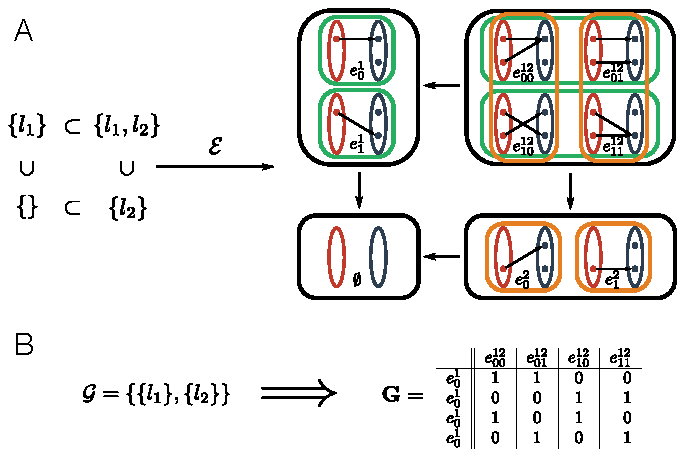
\includegraphics[width=0.8\columnwidth]{fig/efunctor.pdf}
\caption{{\bf Example of the functor mapping subsets of variables to measurable spaces.} (A) On the left hand side are subsets of $L=\{l_1,l_2\}$ ordered by inclusion. On the right hand side are the spaces of \gnpm{} also ordered by inclusion. The labels for the maps define them. For example, $e^{12}_{01}(l_1) = 0$ and $e^{12}_{01}(l_2) = 1$. (B) For the given covering, $\mathcal{G}$, the associated marginalization matrix acting on the probability vector $\{ p^{12}_{00},p^{12}_{01},p^{12}_{10},p^{12}_{11} \}$ to give $\{ p^{1}_{0},p^{1}_{1},p^{2}_{0},p^{2}_{1} \}$ is $\mathbf{G}$.}
\label{fig:efunctor}
\end{figure}

\pagebreak

\begin{figure}[!ht]
\centering
\noindent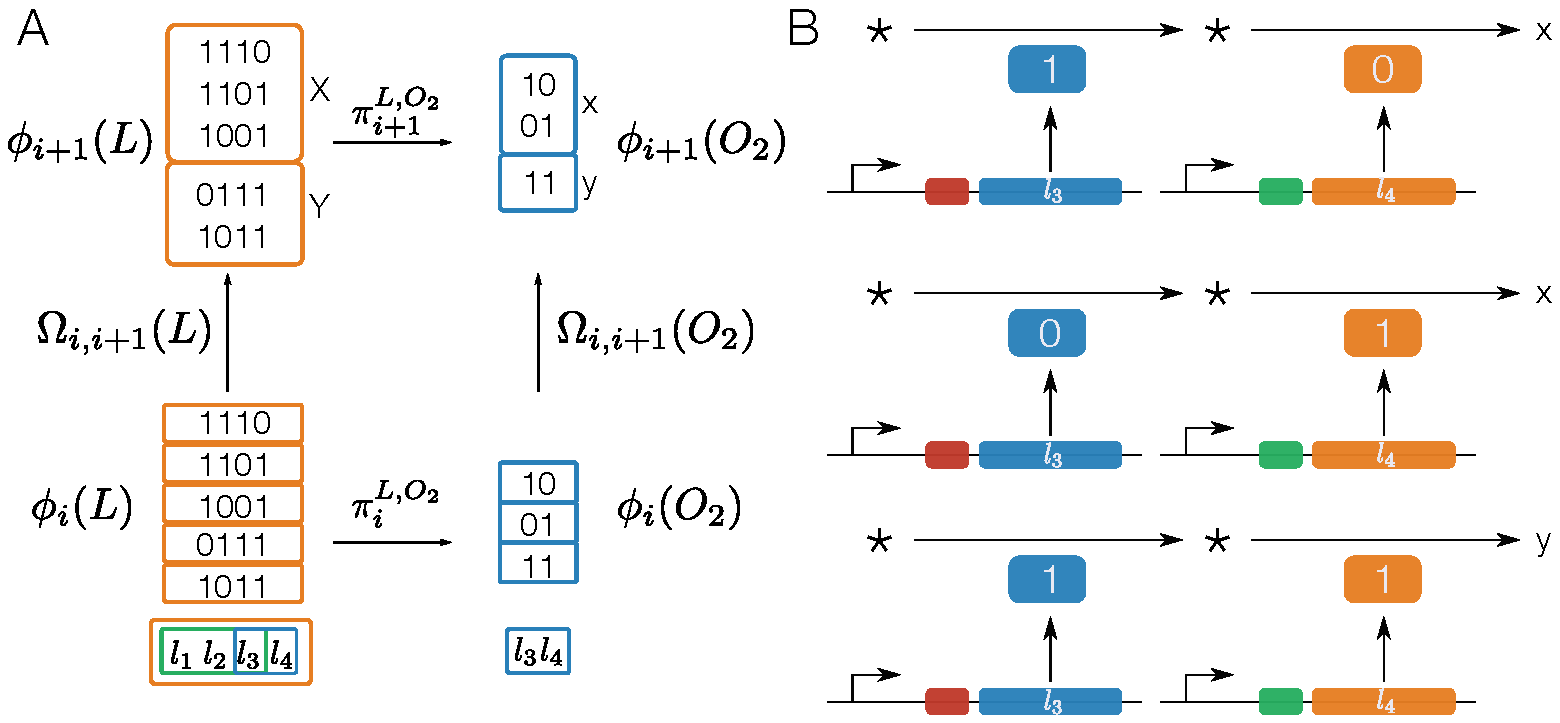
\includegraphics[width=0.9\columnwidth]{fig/phenotypehierarchy.pdf}
\caption{{\bf Example coarse-graining of phenotypes.} (A) Consider the example where $L = \{l_1,l_2,l_3,l_4\}$, $\mathcal{G} = \{ O_1, O_2 \}$, $O_1 = \{l_1, l_2, l_3\}$ and $O_2 = \{ l_3, l_4 \}$. The top left panel shows two higher-level phenotypes $X$ and $Y$. The bottom left corner shows the five different expression states of four genes in $L$ from which these phenotypes are coarse-grained. The right side shows the respective projections onto genes $\{l_3,l_4\}$. The projection maps $\pi_i^{L,O_2}$ and $\pi_{i+1}^{L,O_2}$ are defined in \refsupp{} \ref{secsupp:coarsegrainingphenotypes}. (B) The different combinations of expression states of genes $\{l_3,l_4\}$ result in two different phenotypes. If both genes are expressed metabolite $y$ is produced whereas if only one of the two genes is expressed metabolite $x$ is produced. The red and green boxes represent arbitrary promoters.}
\label{fig:phenotypehierarchy}
\end{figure}

\pagebreak

\begin{figure}[!ht]
\centering
\noindent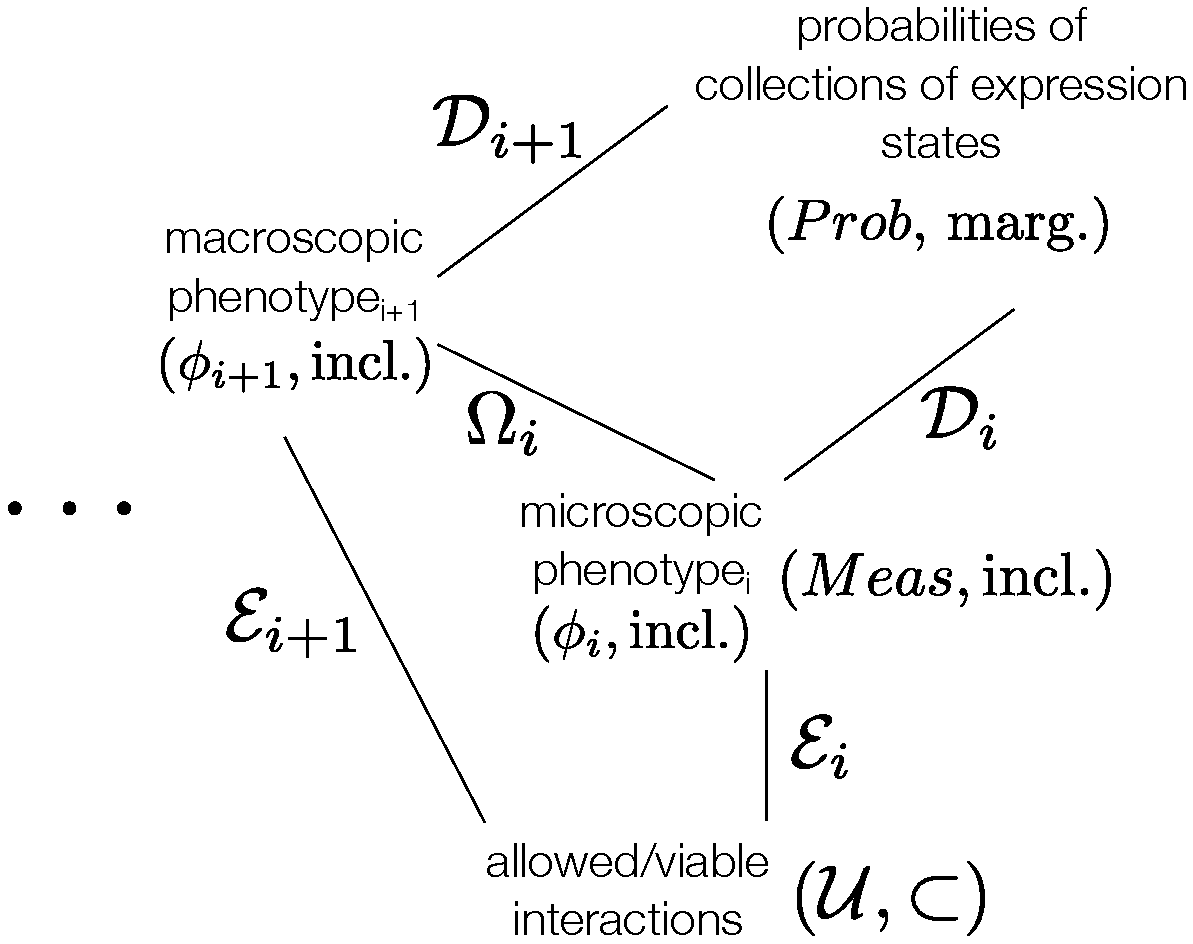
\includegraphics[width=0.4\columnwidth]{fig/abstractroadmap.pdf}
\caption{{\bf Mathematical relationships defining the hierarchy of network states via coarse-graining.} }
\label{fig:abstractroadmap}
\end{figure}

\pagebreak

\begin{figure}[!ht]
\centering
\noindent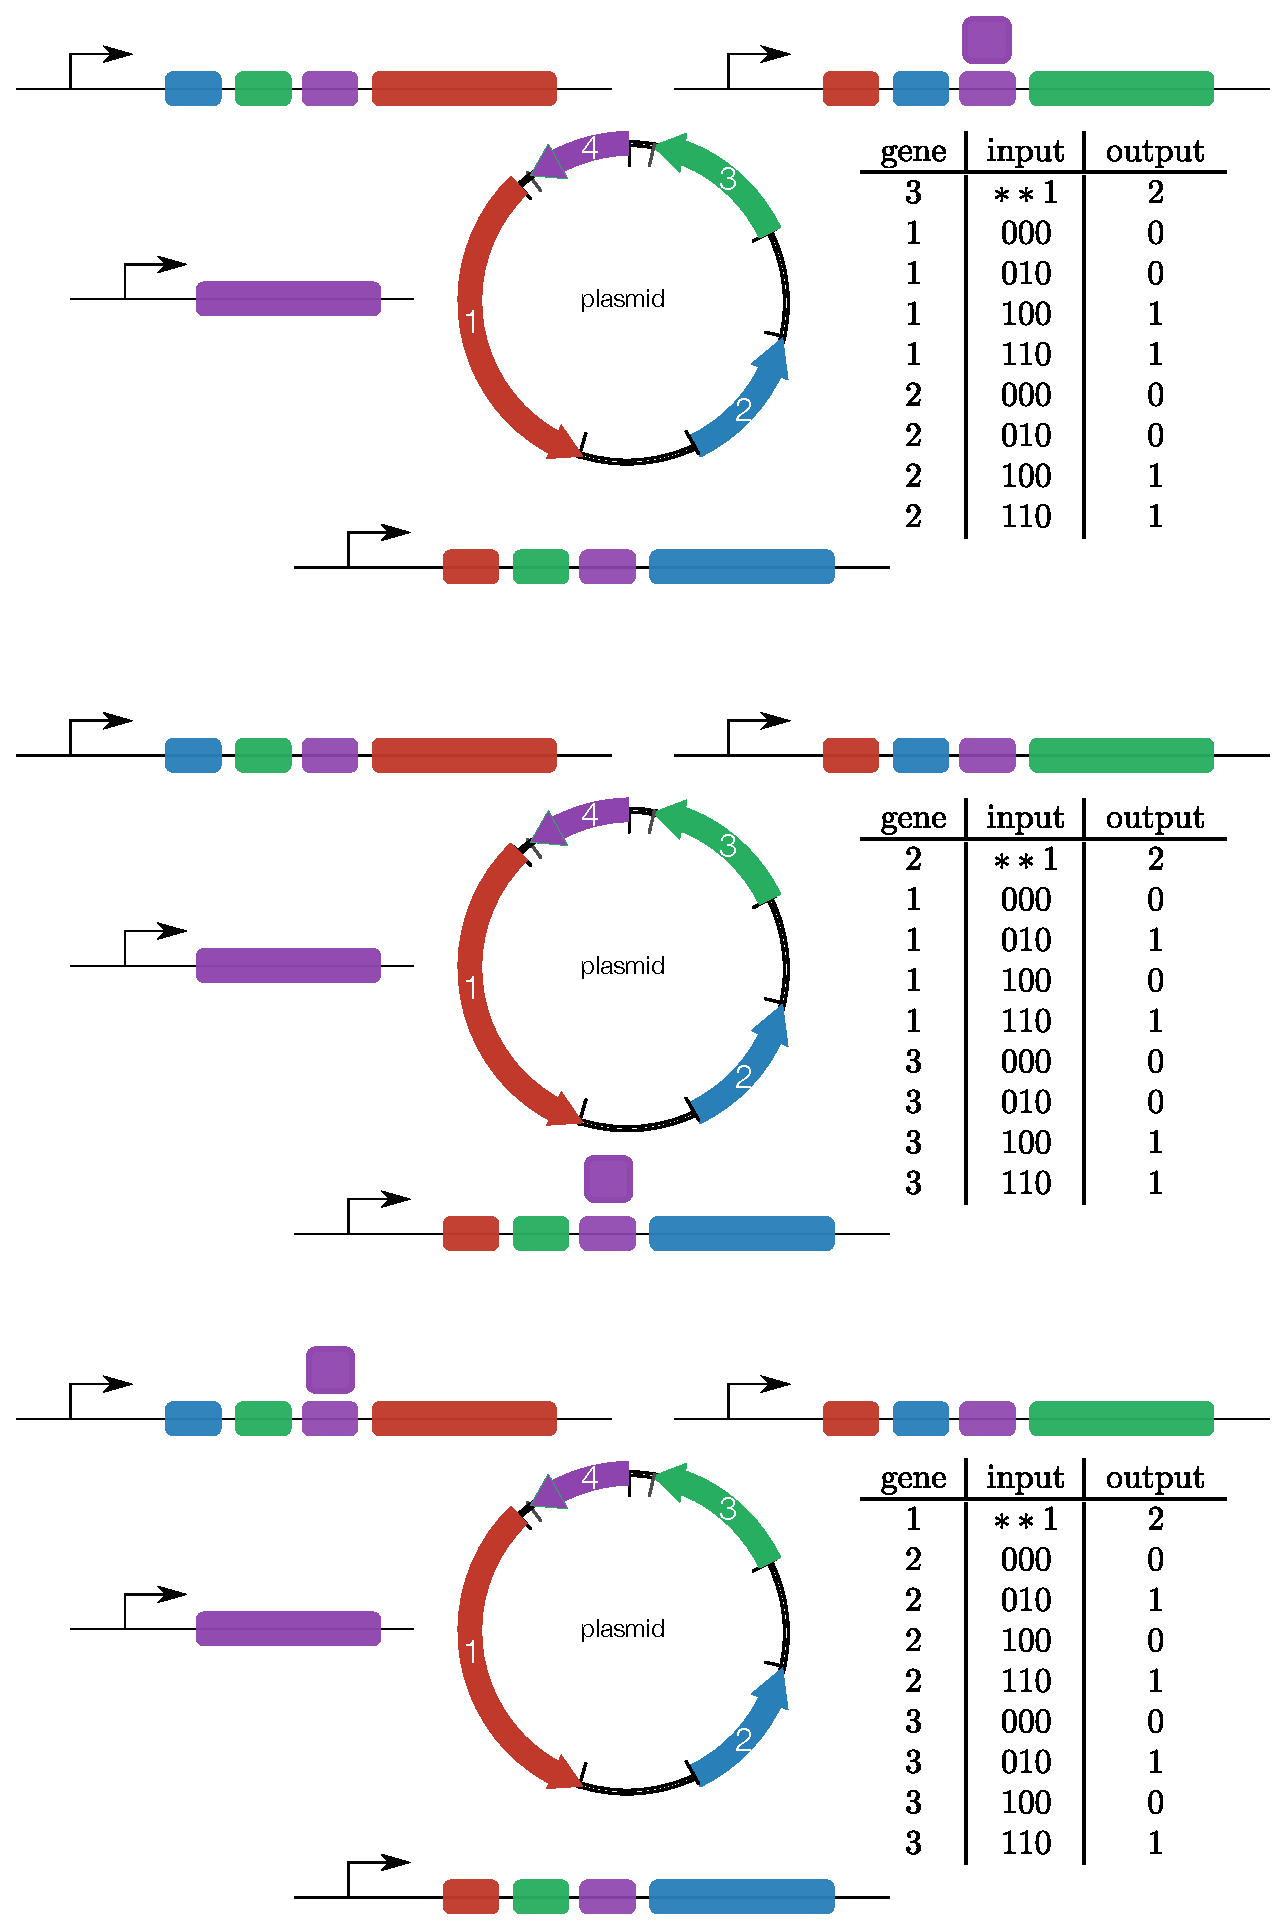
\includegraphics[width=1.0\columnwidth]{fig/condgenescenario.pdf}
\caption{{\bf Schematic synthetic gene circuit capable of exhibiting apparent inconsistency.} A synthetic gene circuit consisting of four genes possesses one gene (purple) whose product is assumed to be present at low copy number and binds randomly with equal affinity to operator sites existing within the operons of each of the other three genes (red, blue, and green). These latter three genes each possess operator sites for the other two, but do not possess autoregulatory operators. They also each exhibit three states represented by three dynamical modes that may involve intermediates not explicitly represented here \cite{Cai2008,Dolmetsch1998}. If the first gene is bound to the operator of another gene, the output is forced into a zero frequency infinite period, or DC, mode (state 2) regardless of the binding state of the other operators. If the first gene is unbound, then the expression state can be switched between low (state 0) and high (state 1) frequency modes depending upon the binding states of other genes as indicated. Note that operators for each of genes one to three are insensitive to the DC mode. Observing pairs of genes one to three and ignoring the state corresponding to the DC mode can lead to apparent inconsistency.}
\label{fig:condgenescenario}
\end{figure}


% \pagebreak

% \begin{figure}[!ht]
% \centering
% \noindent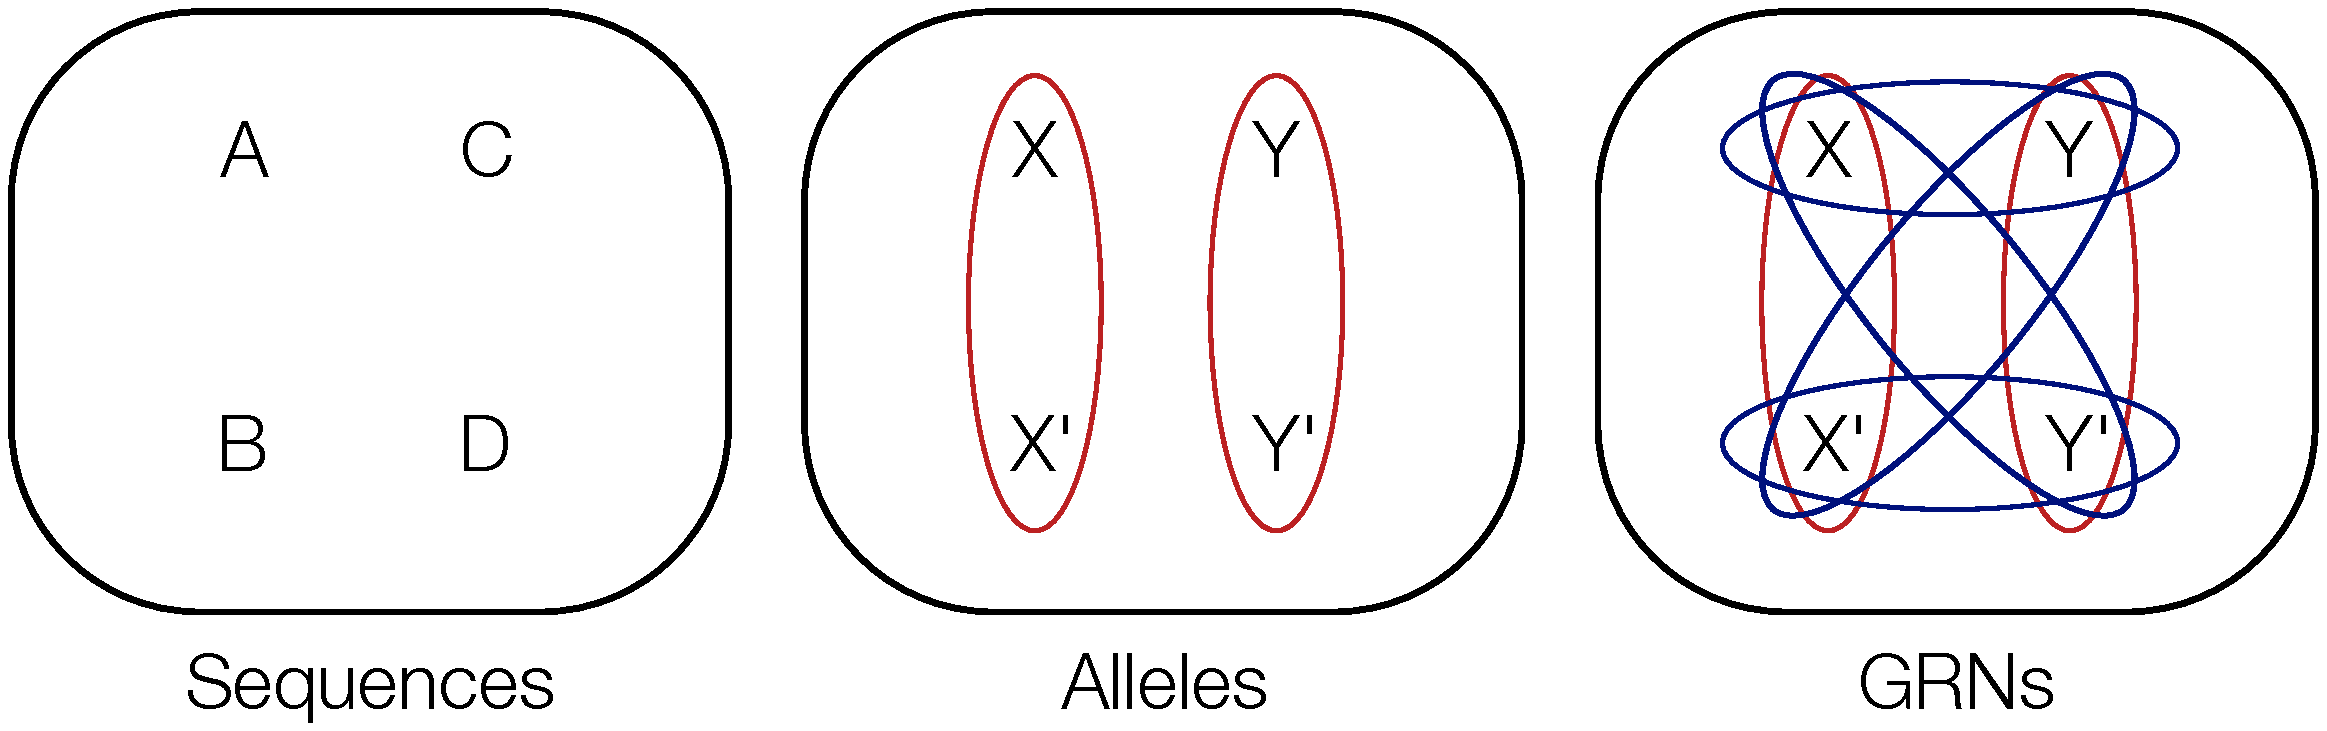
\includegraphics[width=0.7\columnwidth]{fig/genesallelesgrns.pdf}
% \caption{{\bf Sequences, partitions, and GRNs.} In the sequences panel, we consider the letters to be abstract labels for arbitrary genetic sequences that may or may not be found to have a particular function once genetic interactions are taken into account. Sequences may be grouped together, for example if they appear mutually exclusively in gene regulatory networks, under identifications such as~$A=X,\,B=X',\,C=Y,\,D=Y'$. Genomes could then, for example, take one gene from each subset of sequences, by analogy to the partitions representing alleles and the organisms being haploid with all genes are essential. However, in general, we may consider arbitrary subsets of genes to be able to be included in a genome.}
% \label{fig:genesallelesgrns}
% \end{figure}
% \begin{center}
% 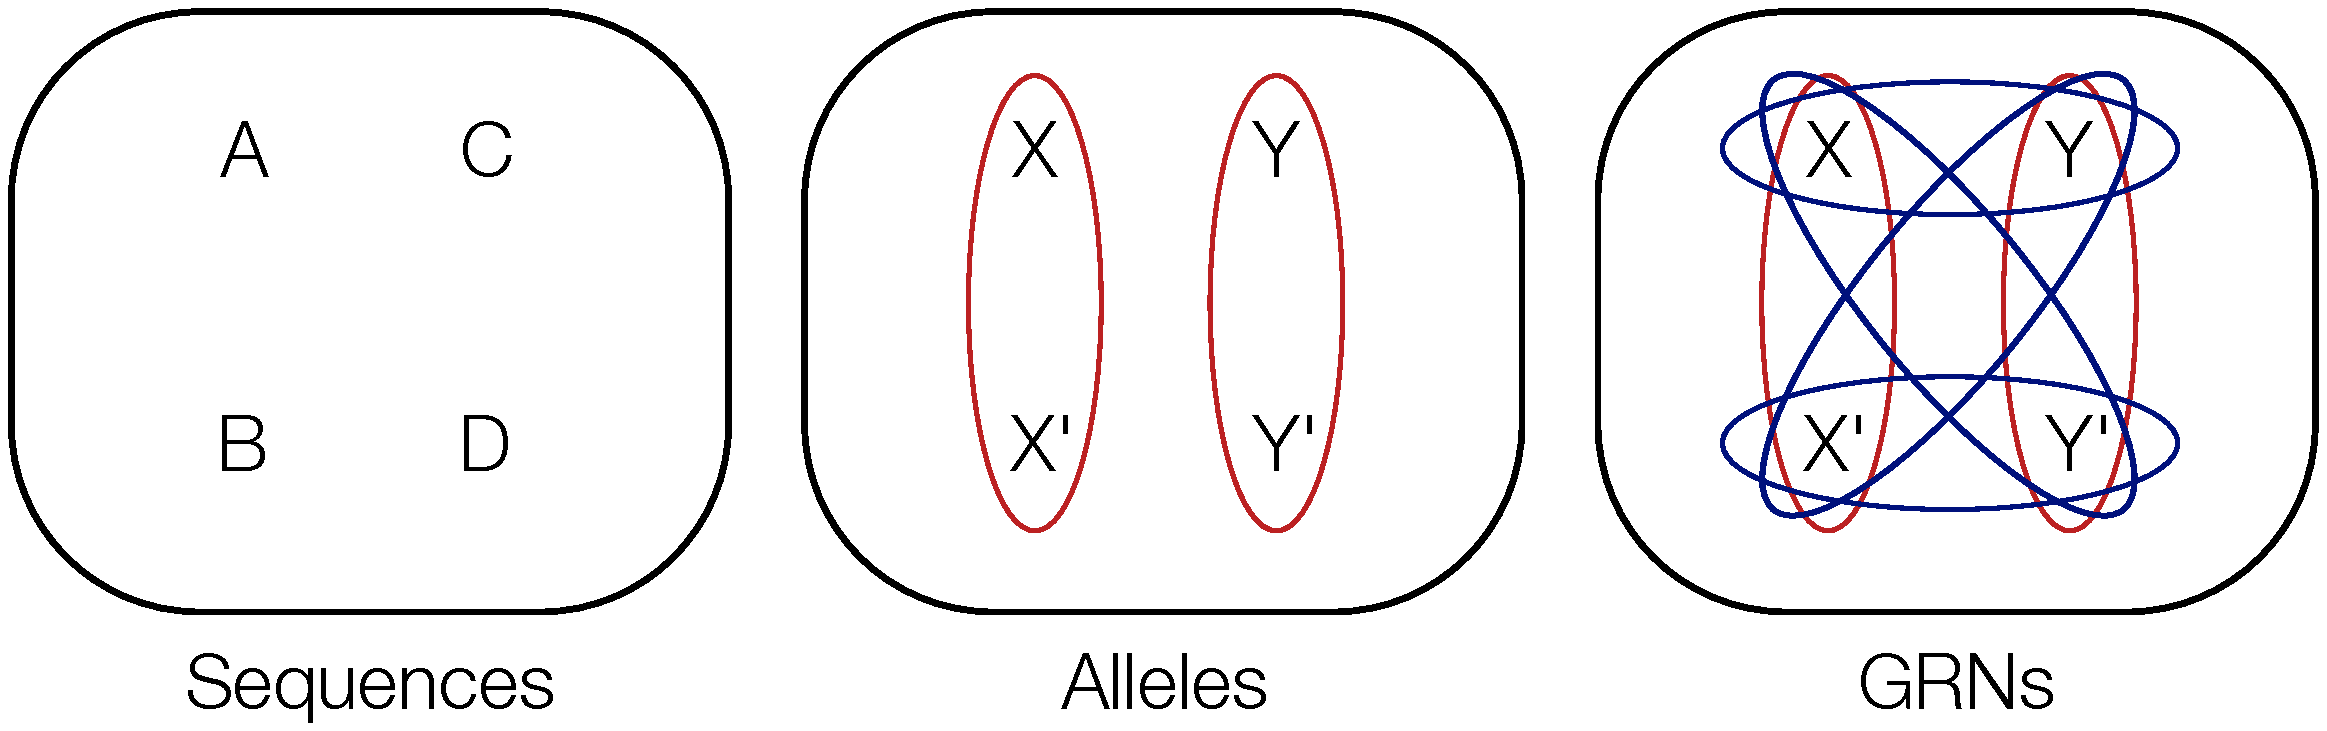
\includegraphics[width=0.9\columnwidth]{fig/genesallelesgrns.pdf}
% \end{center}
% \begin{figure}[!ht]
% \centering
% \noindent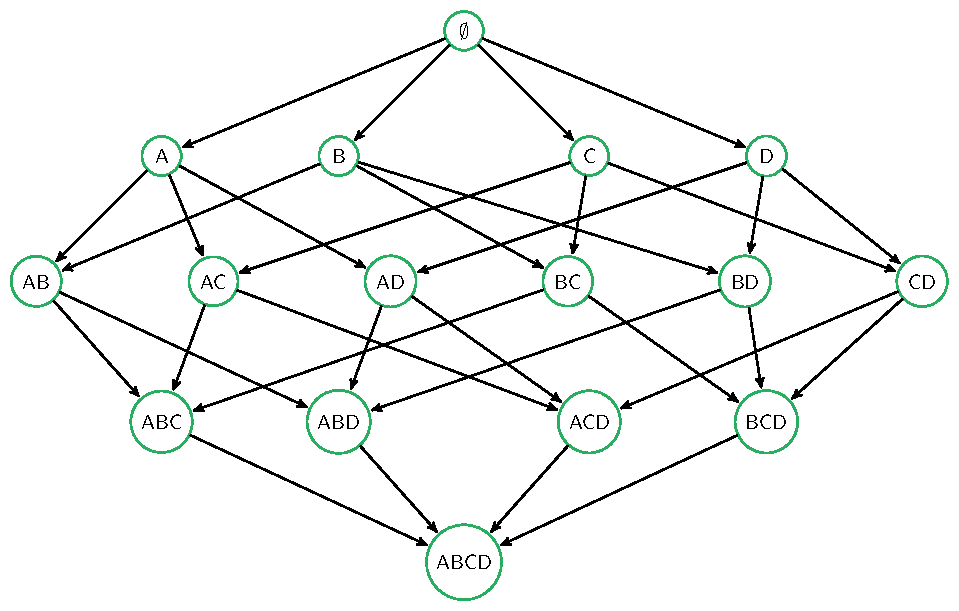
\includegraphics[width=0.4\columnwidth]{fig/potential-interactions.pdf}
% 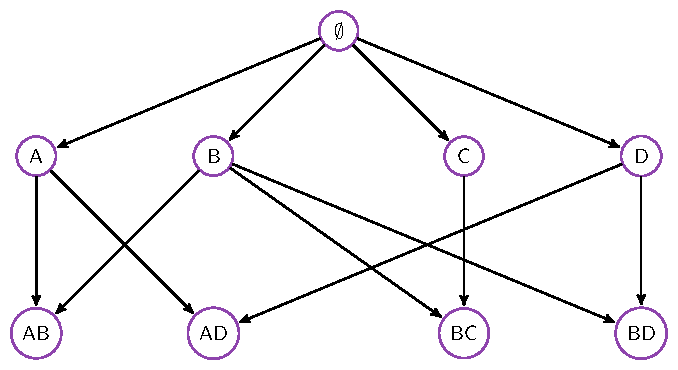
\includegraphics[width=0.4\columnwidth]{fig/two-gene-two-allele-interactions.pdf}
% 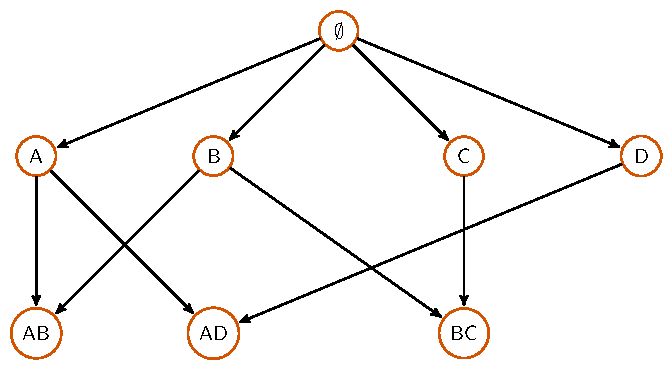
\includegraphics[width=0.4\columnwidth]{fig/incompatibility-interactions.pdf}
% 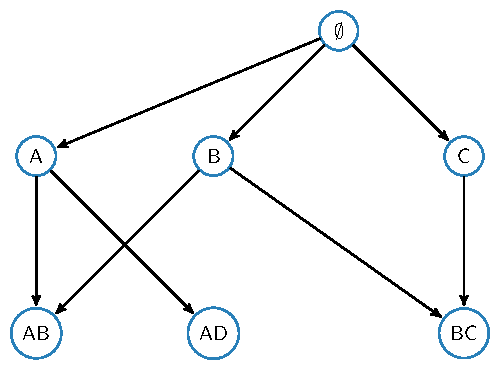
\includegraphics[width=0.4\columnwidth]{fig/dependency-interactions.pdf}
% \caption{{\bf Gene interaction lattices.}}
% \label{fig:geneinteractionlattices}
% \end{figure}
\pagebreak

\begin{figure}[!ht]
\centering
\noindent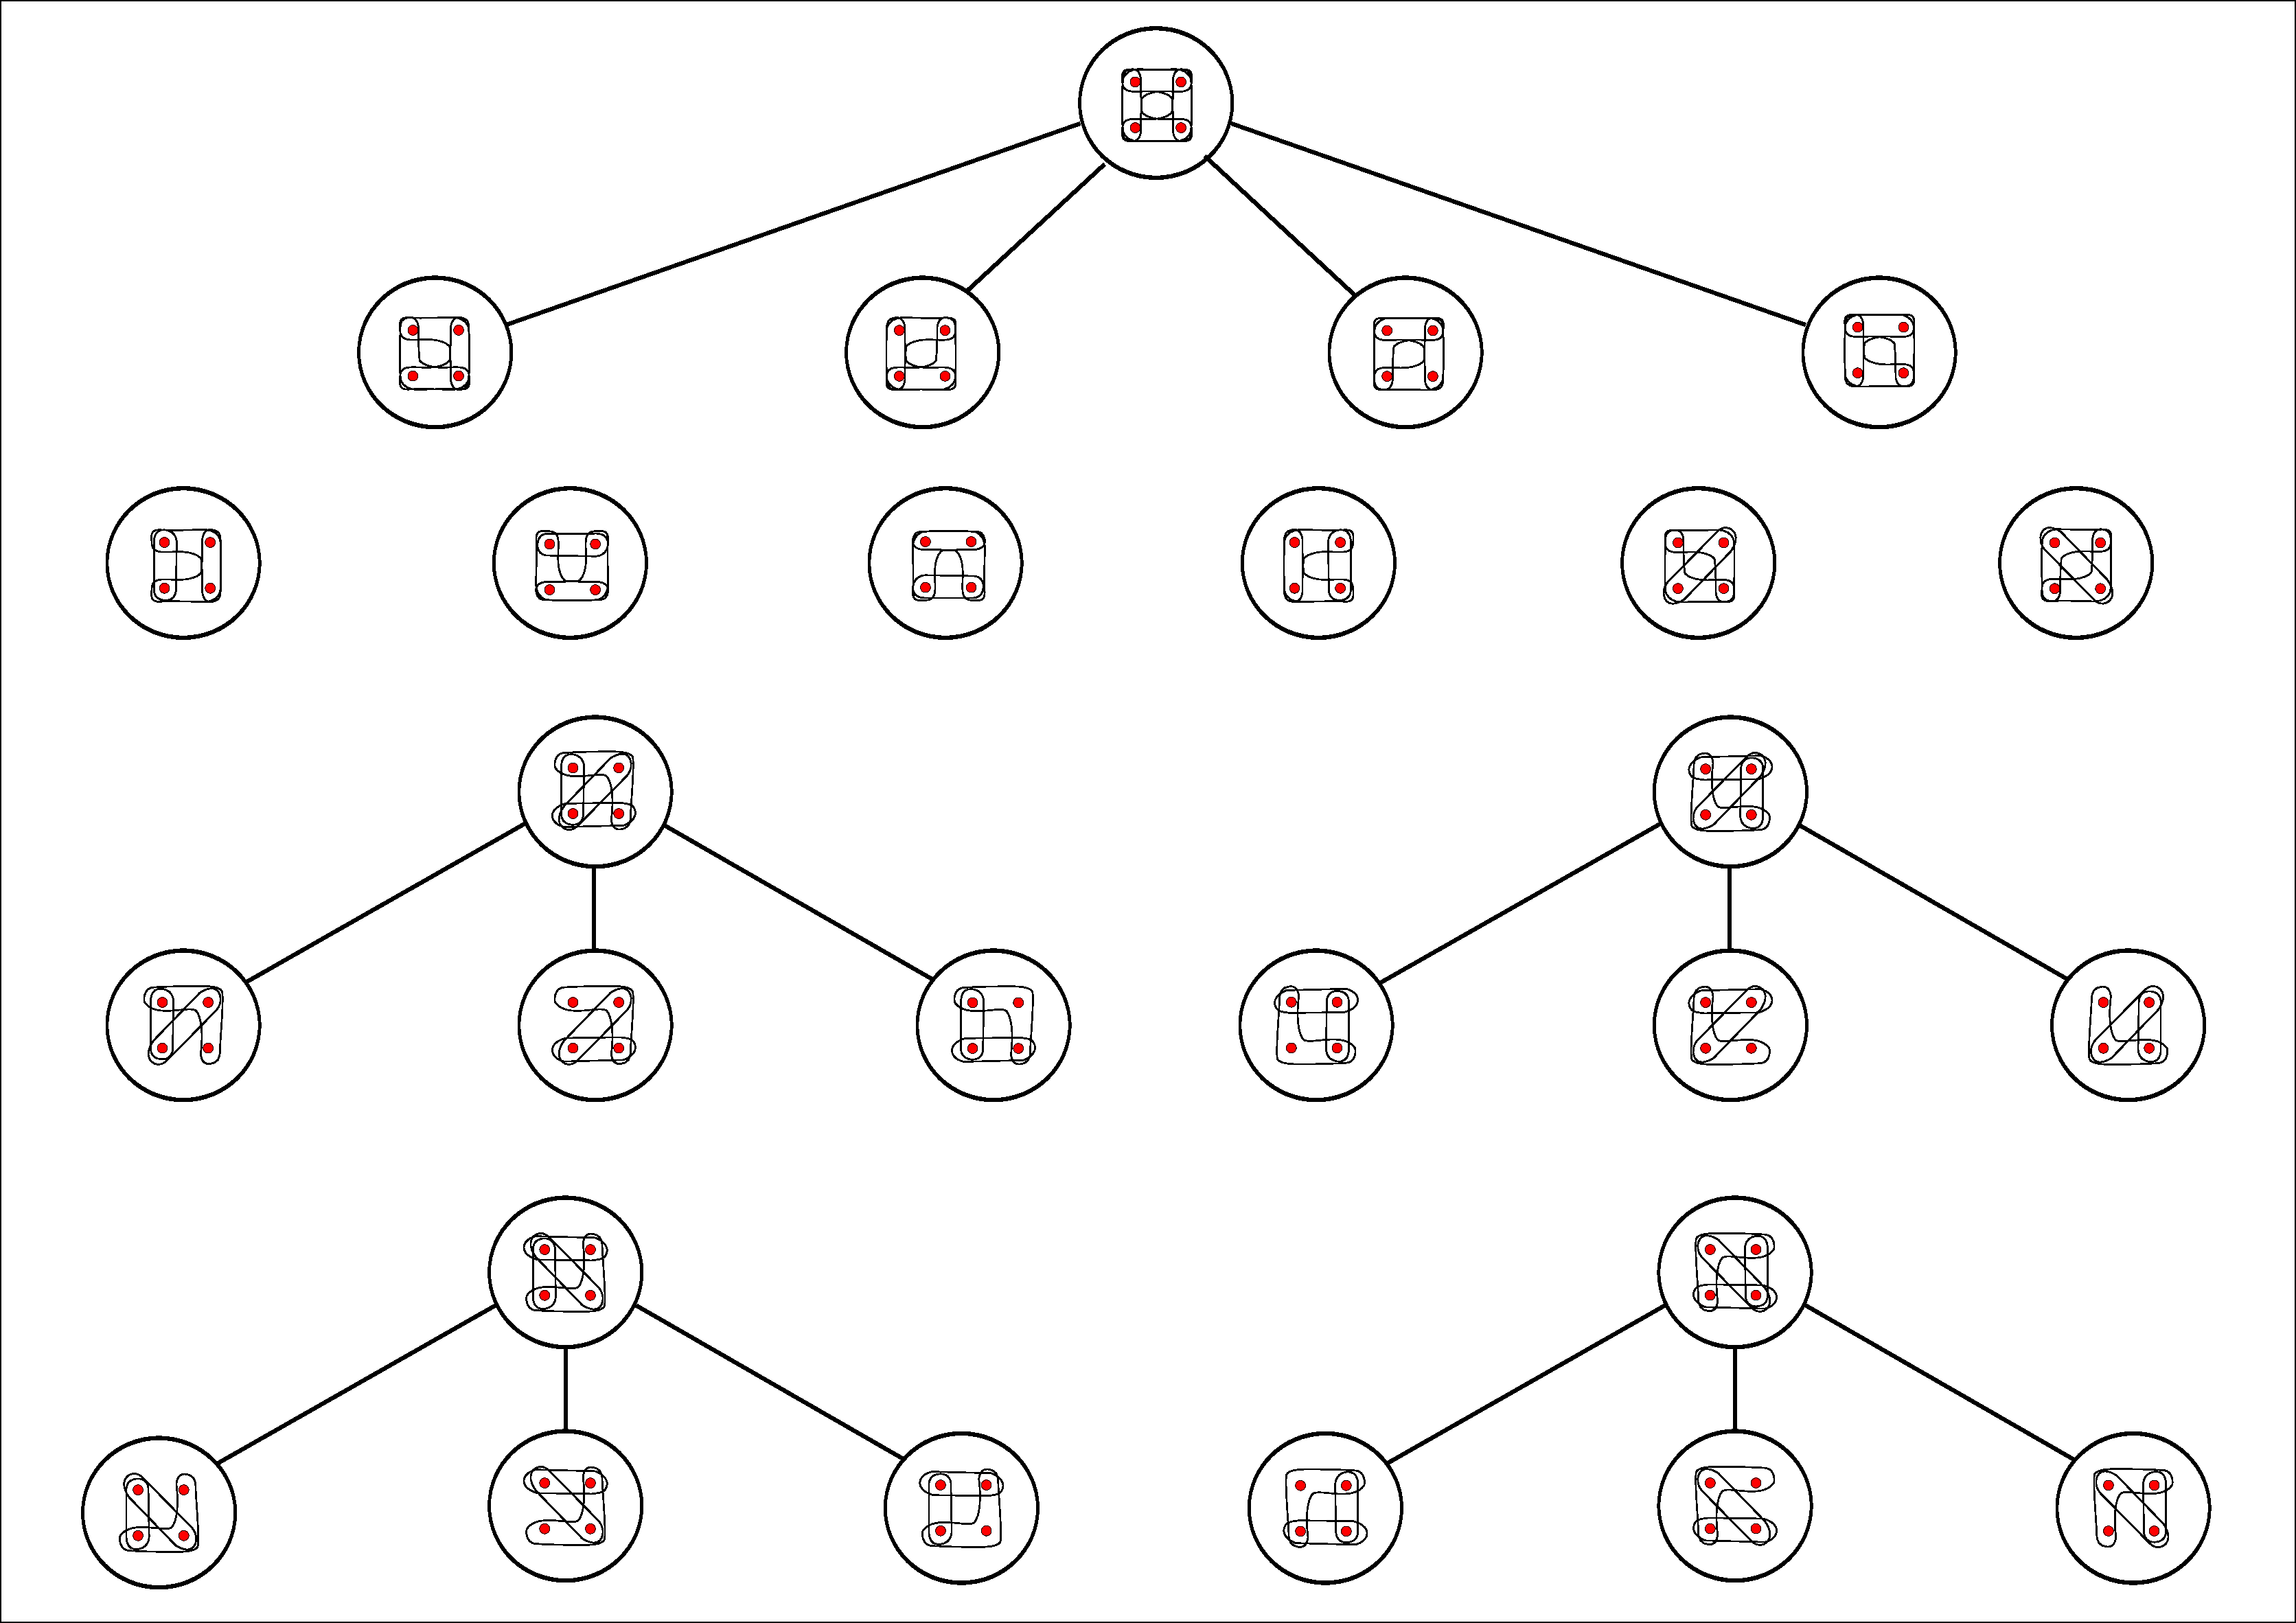
\includegraphics[width=1.0\columnwidth]{fig/non2uniformcyclichypergraphhasse.pdf}
\caption{{\bf Hierarchical relationships among all possible classes of hypergraphs that are not graphs (i.e. not 2-uniform) but have cycles.} (A) There is a Hasse diagram for the lattice of network architectures analogous to that of \ref{fig:conediagram}A but defined on four rather than only three variables. Within this lattice some of the graphs have cycles and some do not. (B) The highest levels of the Hasse diagram associated to the lattice of network architectures on four variables containing hypergraphs having cycles. (C) and (D) contain lower levels of network architectures containing cycles. Each of the four panels in (D) are on the same level. In total, each level represents an isomorphism class of hypergraphs. Therefore, there are five isomorphism classes of non-2-uniform hypergraphs representing network architectures on four variables that contain cycles leading to the relationship between spaces of probability distsributions on associated genotype-phentoype maps analogous to that of \ref{fig:conediagram}C.}
\label{fig:non2uniformcyclichypergraphhasse}
\end{figure}

% \pagebreak

% \begin{figure}[!ht]
% \centering
% \noindent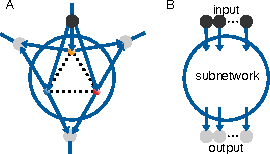
\includegraphics[width=0.3\columnwidth]{fig/controlnetwork.pdf}
% \caption{{\bf Embedding into a particular network context.} The network inside the blue circle is equivalent to that of \ref{fig:inconsistentthreecycle}A, embedded into a particular network context that provides inputs (dark gray node) and outputs (light gray nodes) to the focal subnetwork. As a result of their connectivity, the outputs depend here upon pairwise correlations within the three genes comprising the focal subnetwork.}
% \label{fig:controlnetwork}
% \end{figure}

% \pagebreak

% \begin{figure}[!ht]
% \centering
% \noindent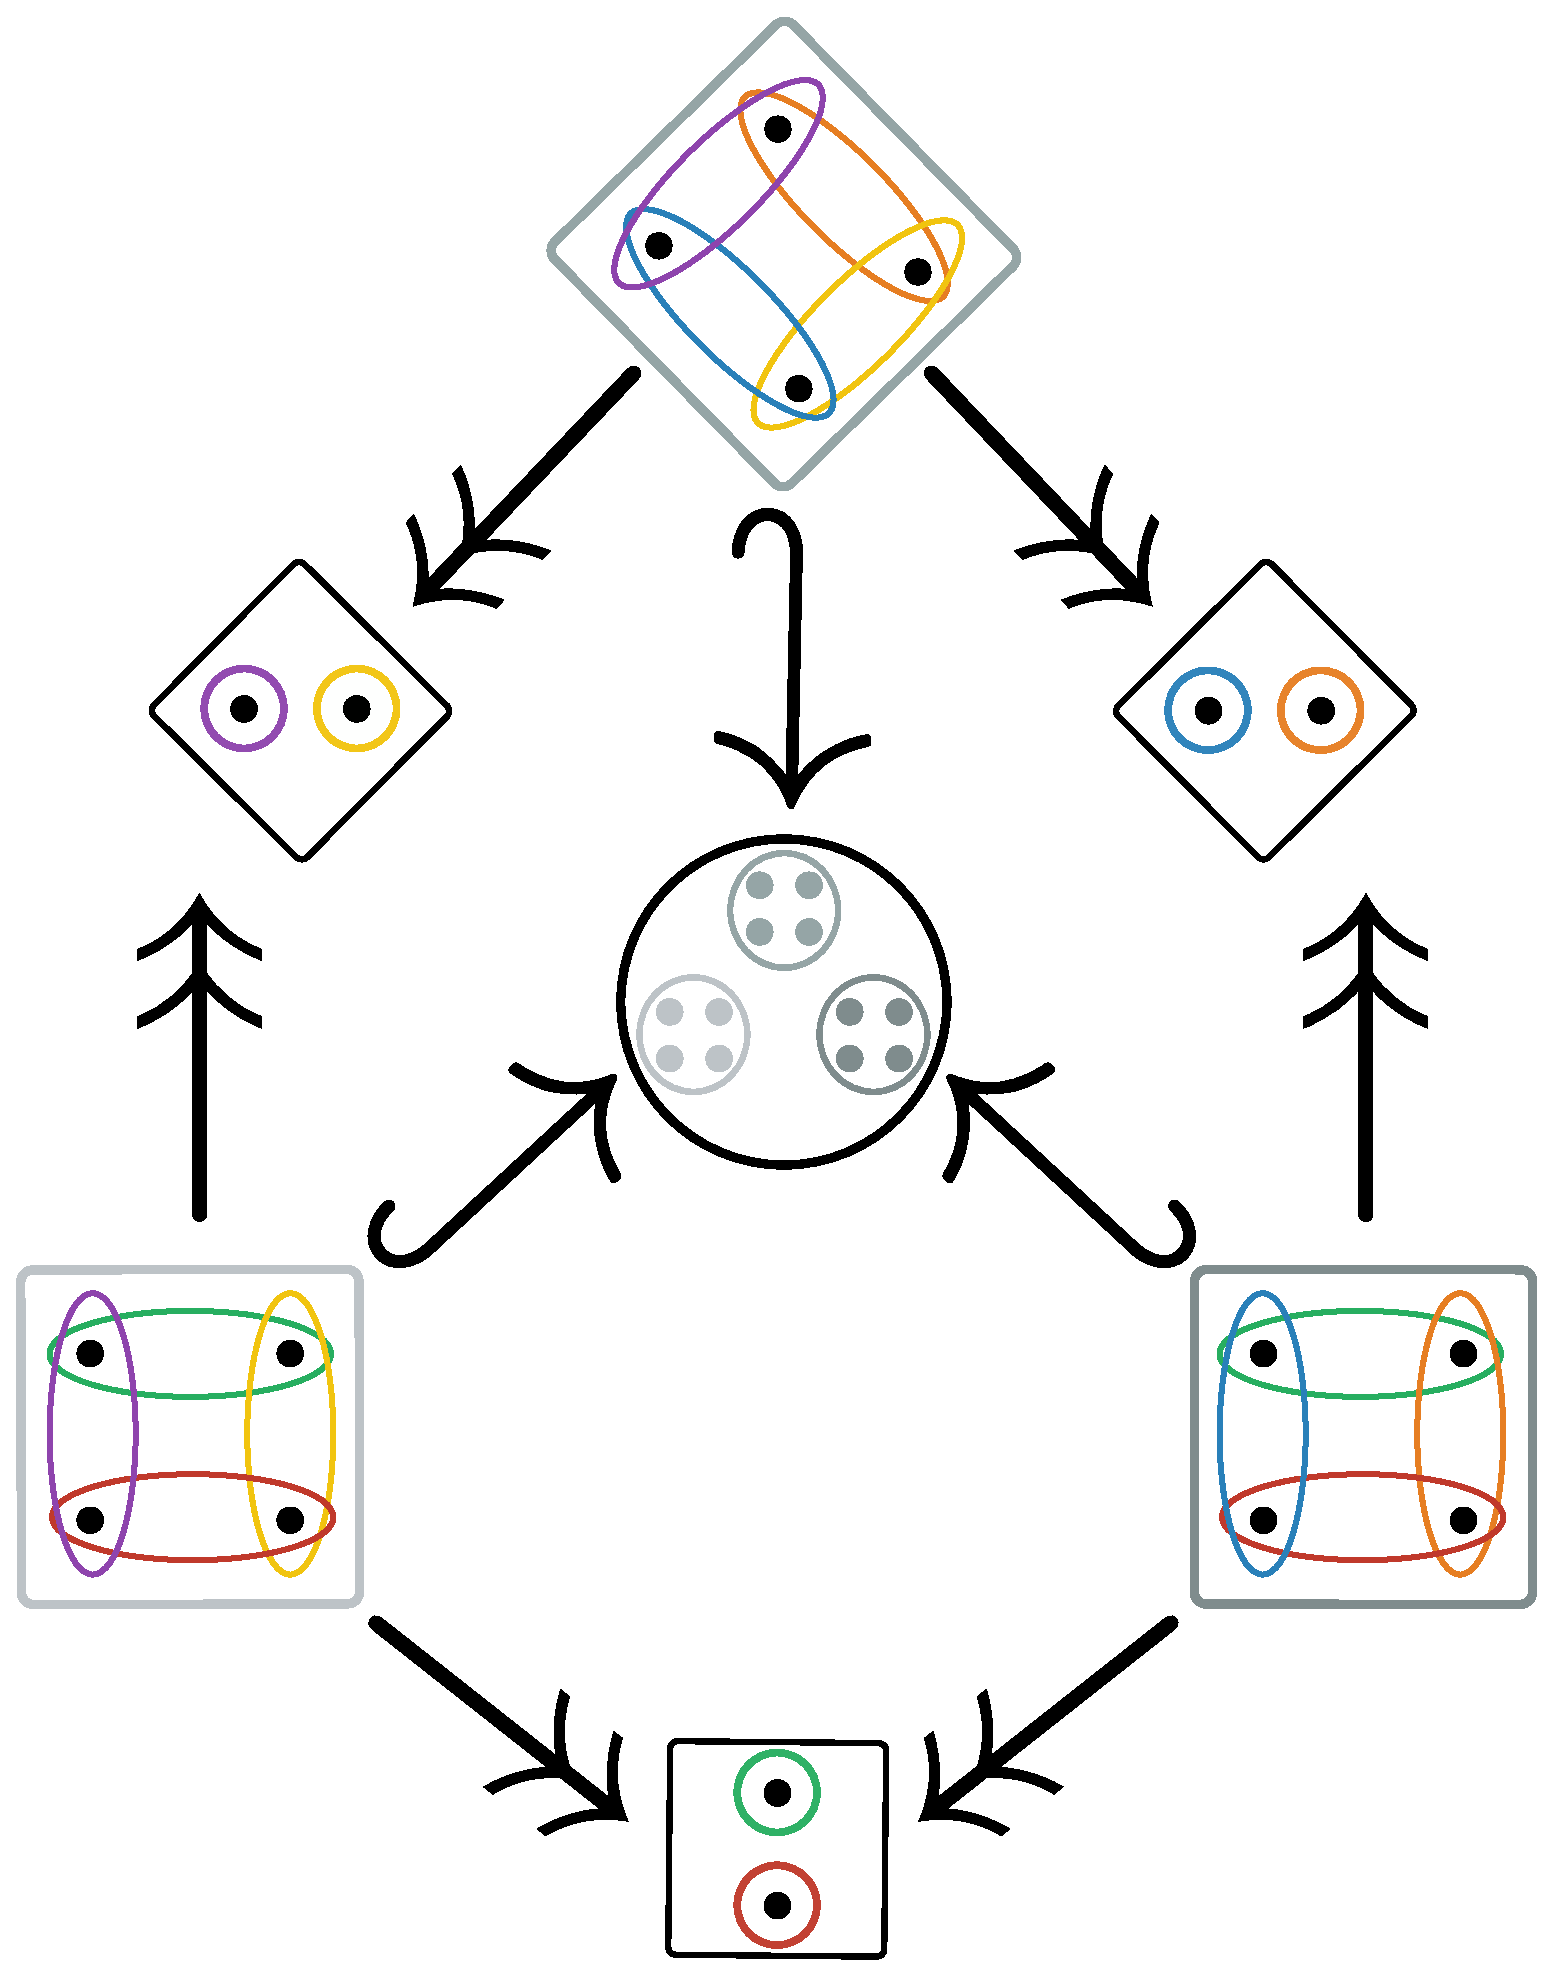
\includegraphics[width=0.5\columnwidth]{fig/condmargprobspaces.pdf}
% \caption{{\bf Diagrammatic representation of the sample spaces for the process generating apparent inconsistency.}}
% \label{fig:condmargprobspaces}
% \end{figure}
